%% iptemplate.tex 
%%
%%   This file is part of the files in the distribution of AIP substyles for REVTeX4.
%%   Version 4.1 of 9 October 2009.
%%
%
% This is a template for producing documents for use with 
% the REVTEX 4.1 document class and the AIP substyles.
% 
% Copy this file to another name and then work on that file.
% That way, you always have this original template file to use.
% chktex-file 36
\documentclass[aip,graphicx]{revtex4-1} % chktex 8
%\documentclass[aip,reprint]{revtex4-1}
\usepackage{amsmath}
\usepackage[utf8]{inputenc}
\usepackage{graphicx}
\usepackage{xcolor}
\renewcommand{\thefigure}{S\arabic{figure}}
%\usepackage{siunitx}
\def\ontop#1#2{\genfrac{}{}{0pt}{}{#1}{#2}}
% chktex-file 35
\draft% marks overfull lines with a black rule on the right

\begin{document}

% Use the \preprint command to place your local institutional report number 
% on the title page in preprint mode.
% Multiple \preprint commands are allowed.
%\preprint{}

\title{Magnetic-field Assisted Assembly of Colloidal Ellipsoids}

% repeat the \author .. \affiliation  etc. as needed
% \email, \thanks, \homepage, \altaffiliation all apply to the current author.
% Explanatory text should go in the []'s, 
% actual e-mail address or url should go in the {}'s for \email and \homepage.
% Please use the appropriate macro for the type of information

% \affiliation command applies to all authors since the last \affiliation command. 
% The \affiliation command should follow the other information.

%\author{}

\author{Antara Pal}
\email{antara.pal@fkem1.lu.se}
\affiliation{Division of Physical Chemistry, Department of Chemistry, Lund University, Lund, Sweden}
\author{Carlo Andrea De Filippo}
\affiliation{Science Department, University Roma Tre, Via della Vasca Navale 84, Roma, Italy}
\author{Thiago H.Ito}
\affiliation{Division of Physical Chemistry, Department of Chemistry, Lund University, Lund, Sweden}
\author{Md. Arif Kamal}
\affiliation{Centre Interdisciplinaire de Nanoscience de Marseille (CINaM), CNRS, Aix Marseille University, Marseille, France}
\altaffiliation[Current Address: ]{Division of Physical Chemistry, Department of Chemistry, Lund University, Lund, Sweden}
\author{Andrei V. Petukhov}
\affiliation{Van't Hoff Laboratory for Physical and Colloid Chemistry, Utrecht University, The Netherlands}
\author{Cristiano De Michele}
\affiliation{Department of Physics, Universit\`{a} di Roma La Sapienza, I-00186 Roma, Italy}
\author{Peter Schurtenberger}
\email{peter.schurtenberger@fkem1.lu.se}
\affiliation{Division of Physical Chemistry, Department of Chemistry, Lund University, Lund, Sweden}


% Collaboration name, if desired (requires use of superscriptaddress option in \documentclass). 
% \noaffiliation is required (may also be used with the \author command).
%\collaboration{}
%\noaffiliation

%\date{\today}

%\pacs{}% insert suggested PACS numbers in braces on next line

\maketitle {}%\maketitle must follow title, authors, abstract and \pacs
\section{Characterization of the phase behavior}

\subsection{Real space structure}

%Fig.\ref{paperclip}(a) shows the real space structure of a classical smectic phase consists of rod-like colloids where the particles are aligned along their long axes. As a result, the smectic layers are along their length. Fig.\ref{paperclip}(b) shows the corresponding Fourier space image or the expected x-ray diffraction pattern~\cite{kuijk2012phase, byelov2013situ}. Fig.\ref{paperclip}(c) represents the smectic phase formed by our ellipsoidal particles in the presence of an external field. One can observe that the particles are aligned with their short axes being parallel to the external field. The red doubled arrows show the spacings along the layers. There are also correlations between particles belong to different layers as shown by green lines which result in the formation of a diffused scattering line as shown in Fig.\ref{paperclip}(d) in green. Although from our drawing it seems that the long axes are also aligned, it is not true. In reality they can still rotate around the field as has been shown in Fig. 2. For the drawing, we have not considered all possible rotational conformations but only one; otherwise it will be extremely difficult to draw and point out the different spacings while including the all rotational conformations. Further, The layers in the smectic phase are not rigid but can fluctuate as can be seen in Fig.\ref{paperclip}(e) which elongated the smectic peak in vertical direction as shown by dark yellow in Fig.\ref{paperclip}(f). Combining all the aforementioned effects it is possible to understand the paperclip shape for the smectic phase in our study.

The real space structure of a classical smectic phase consisting of rod-like colloids is schematically shown in Fig.~\ref{paperclip}(a). In this case the
particles align along their long  axes. As a result, the smectic layers form in a direction parallel to the length of the rods. The corresponding Fourier space
image or the expected x-ray diffraction pattern of the aforementioned smectic phase is shown in Fig.~\ref{paperclip}(b)~\cite{kuijk2012phase, byelov2013situ}.
\begin{figure}[]
\centering
\includegraphics[width=0.6\columnwidth]{paperclip.png}
\caption{(a) Real space image of a classical smectic phase formed by colloidal rods and (b) expected x-ray diffraction pattern for it. (c) Real space image of \textit{oblate} smectic phase formed by ellipsoids and (d) expected diffraction x-ray diffraction pattern for it. (e) Smectic phase with layer fluctuation and (d) the corresponding change in the diffraction pattern.}\label{paperclip}
\end{figure}

However, the smectic phase formed by ellipsoidal particles which in the presence of an external field align with their short axes parallel to the external
field, has the appearance as shown in Fig.\ref{paperclip}(c). The double headed red arrows indicate the spacings along the smectic layers. Correlations between
particles which belong to different layers (as indicated by green lines) results in the formation of a diffused scattering line as shown in
Fig.\ref{paperclip}(d) in green. Although our schematic gives an impression that the long axes are also aligned, but this is not the case in general. As
mentioned before the particles align with their short axes along the field direction and their long axes are free to rotate about this direction (Fig. 2). For
the sake of clarity in illustration, we have chosen to
highlight only one such possible conformation out the ensemble of all possible rotational conformations. Further it is important to note that the smectic layers
in this case are not rigid but can fluctuate, Fig.\ref{paperclip}(e), resulting thereby in an elongation of the smectic peak in vertical direction as indicated
by dark yellow in Fig.\ref{paperclip}(f).


\subsection{Static Structure factor}

\begin{figure}
    \centering
    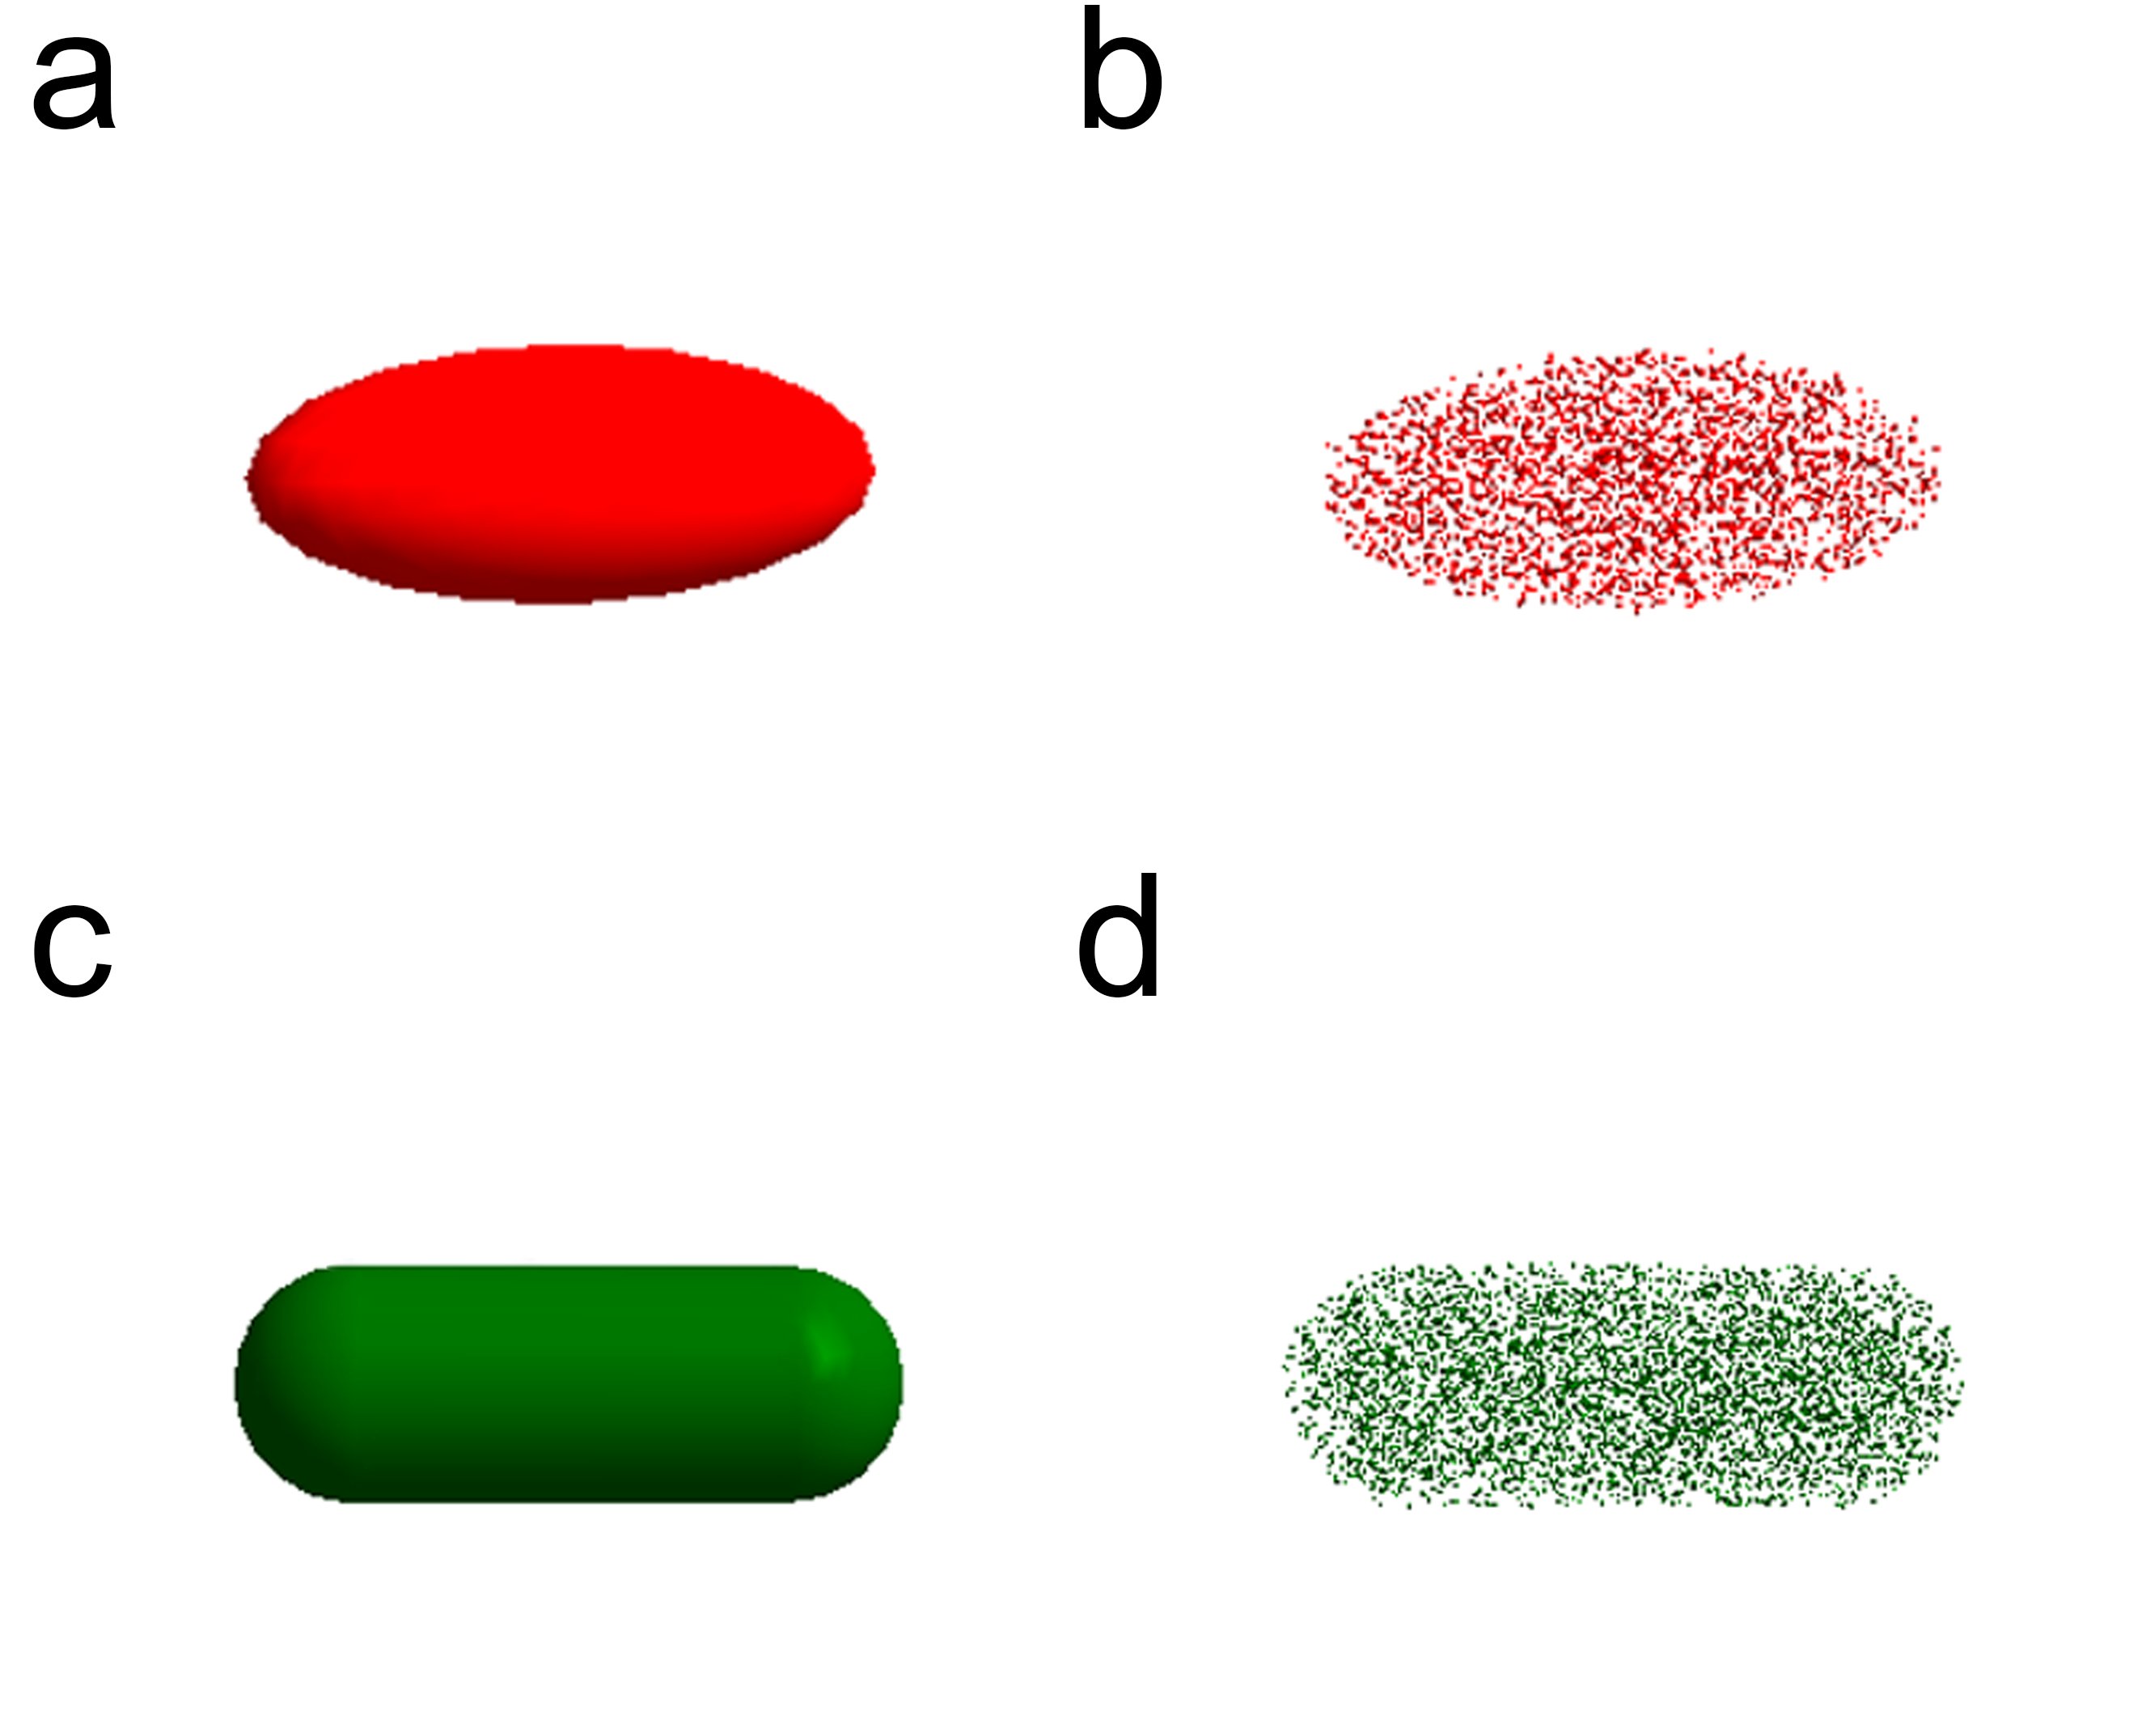
\includegraphics[width=0.4\columnwidth]{Scatteringmodel_single.png}
    \caption{3D representations of a ellipsoid (a) and a spherocylinder (c) and their corresponding random sets of points, shown 
     in panels (b) and (d), respectively.}\label{fig:scatt_mod_single}
\end{figure}

\begin{figure}
    \centering
    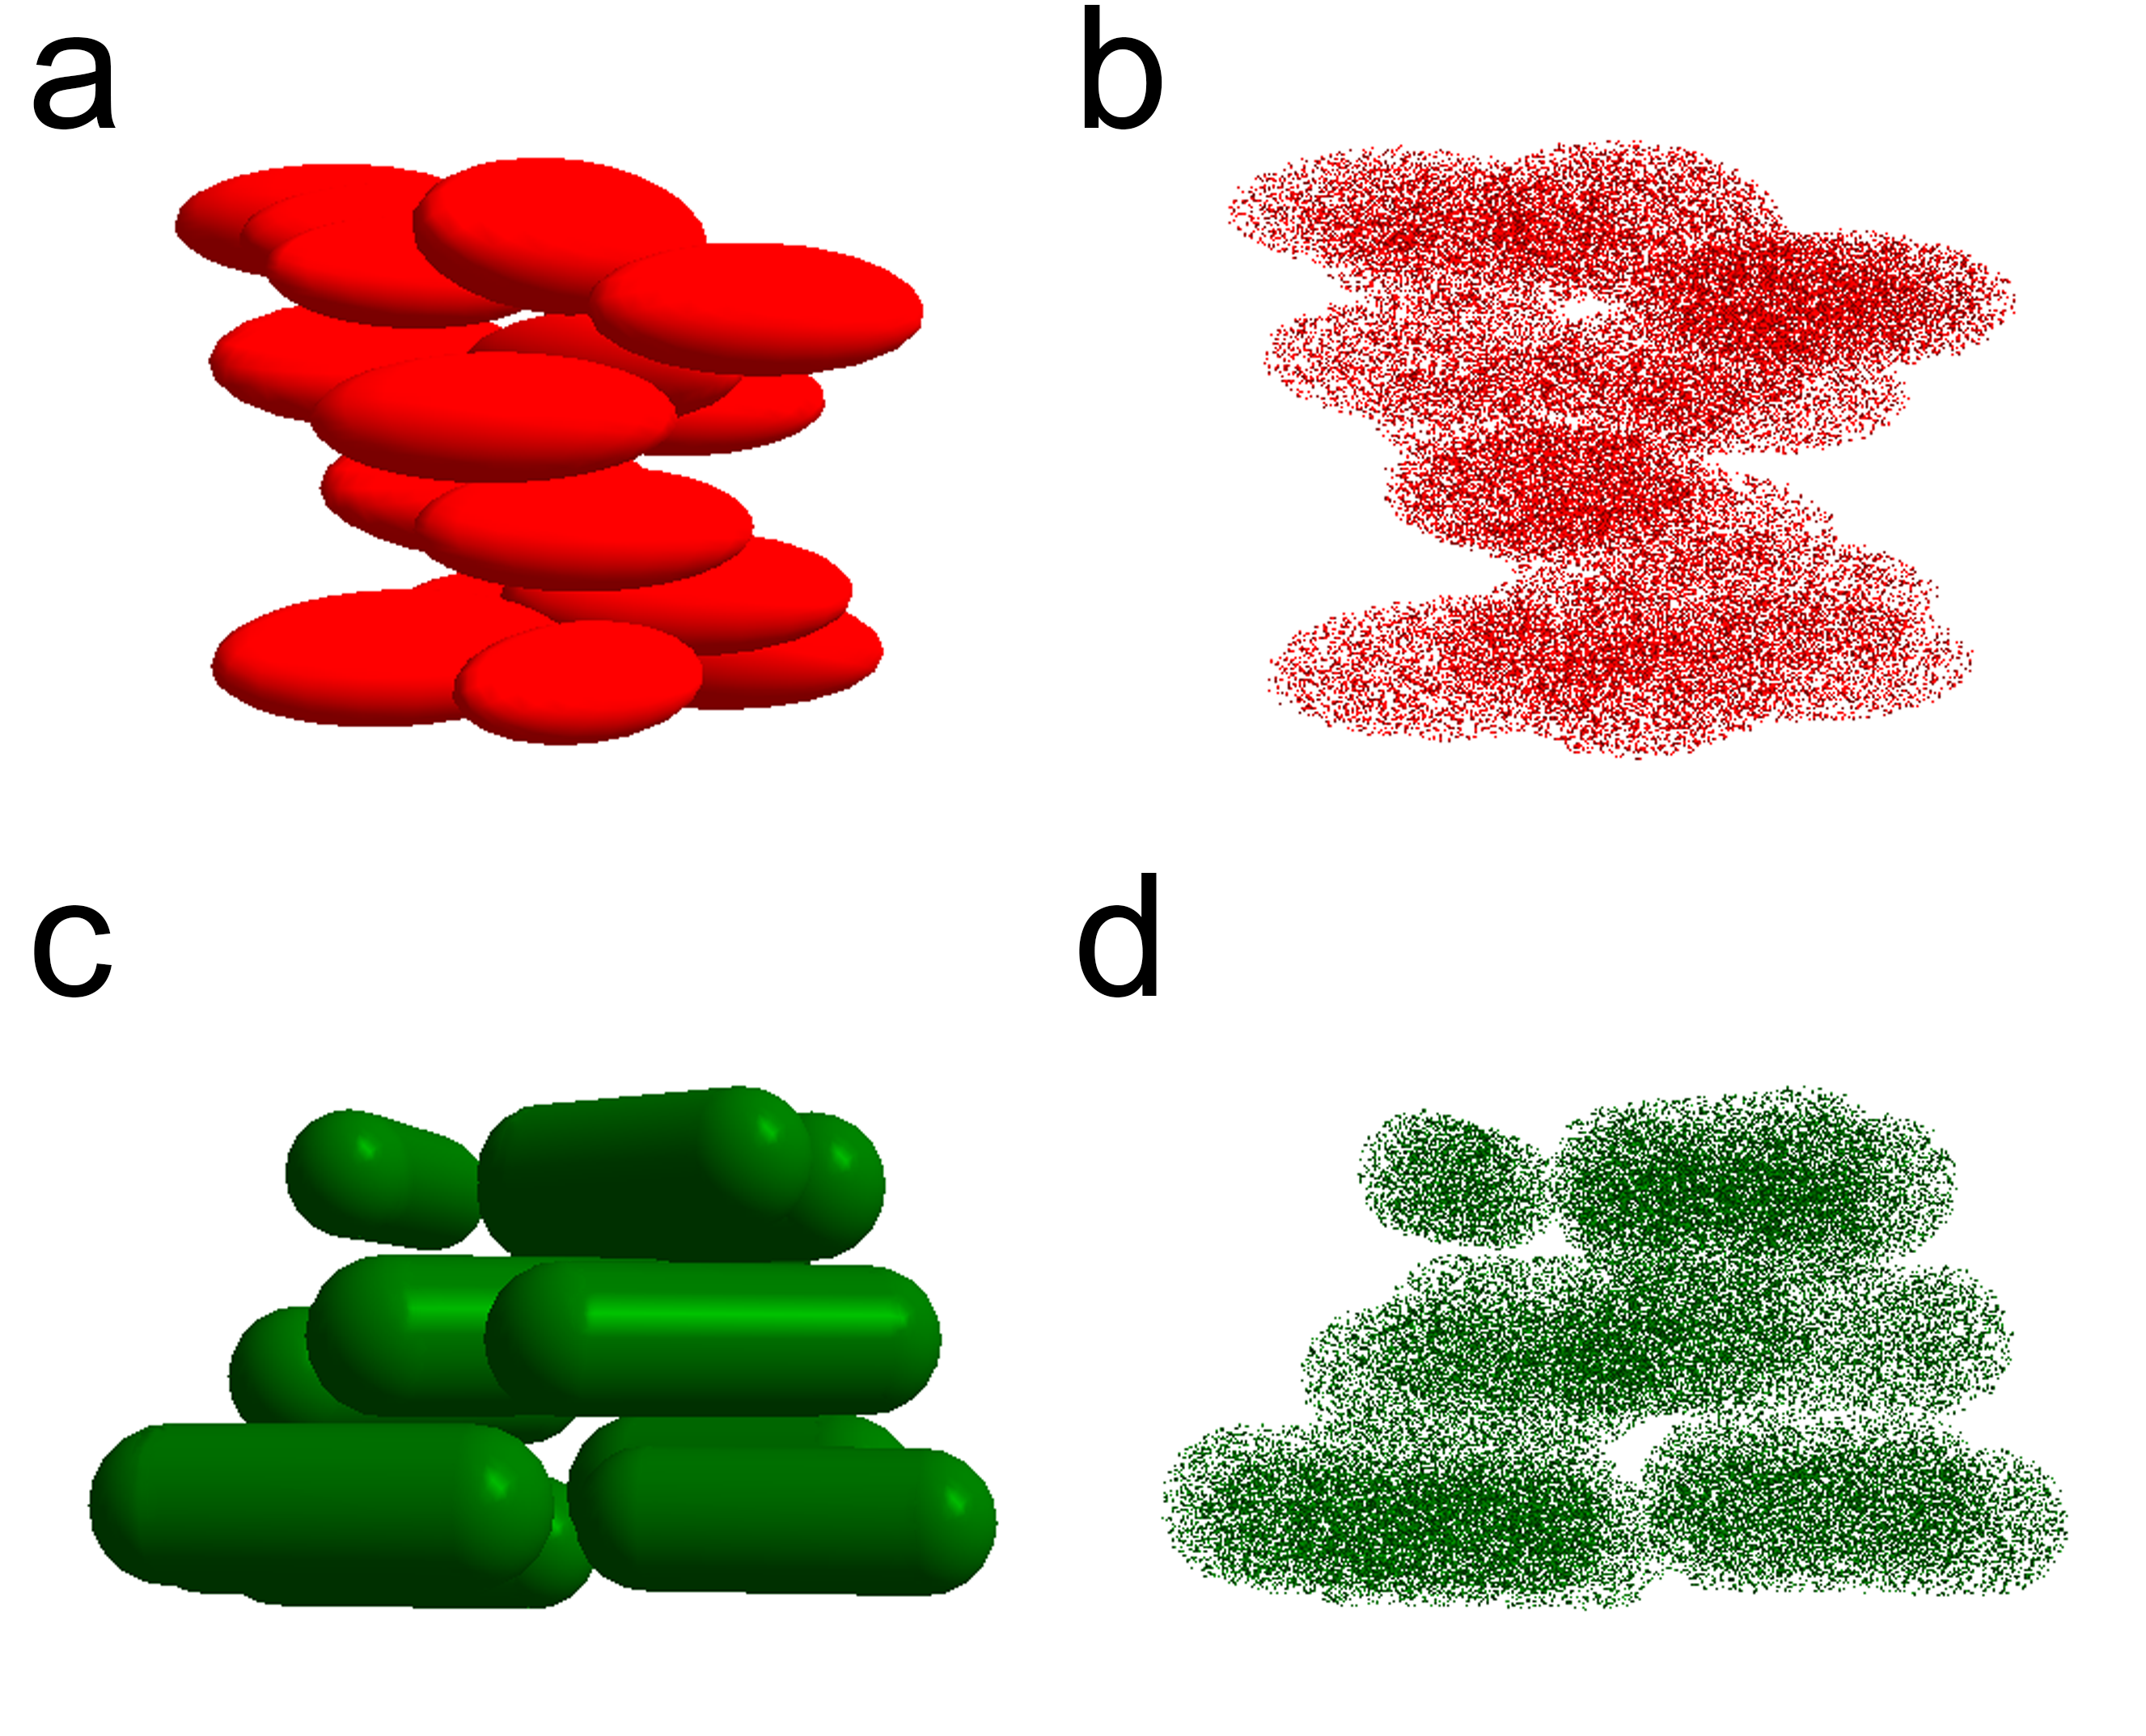
\includegraphics[width=0.4\columnwidth]{Scatteringmodel1.png}
    \caption{A set of HEs (a) and HSCs (c) represented as 3D solids and as random sets of points 
    shown in panels (b) and (d), respectively.}\label{fig:scatt_mod1}
\end{figure}


\begin{figure}
    \centering
    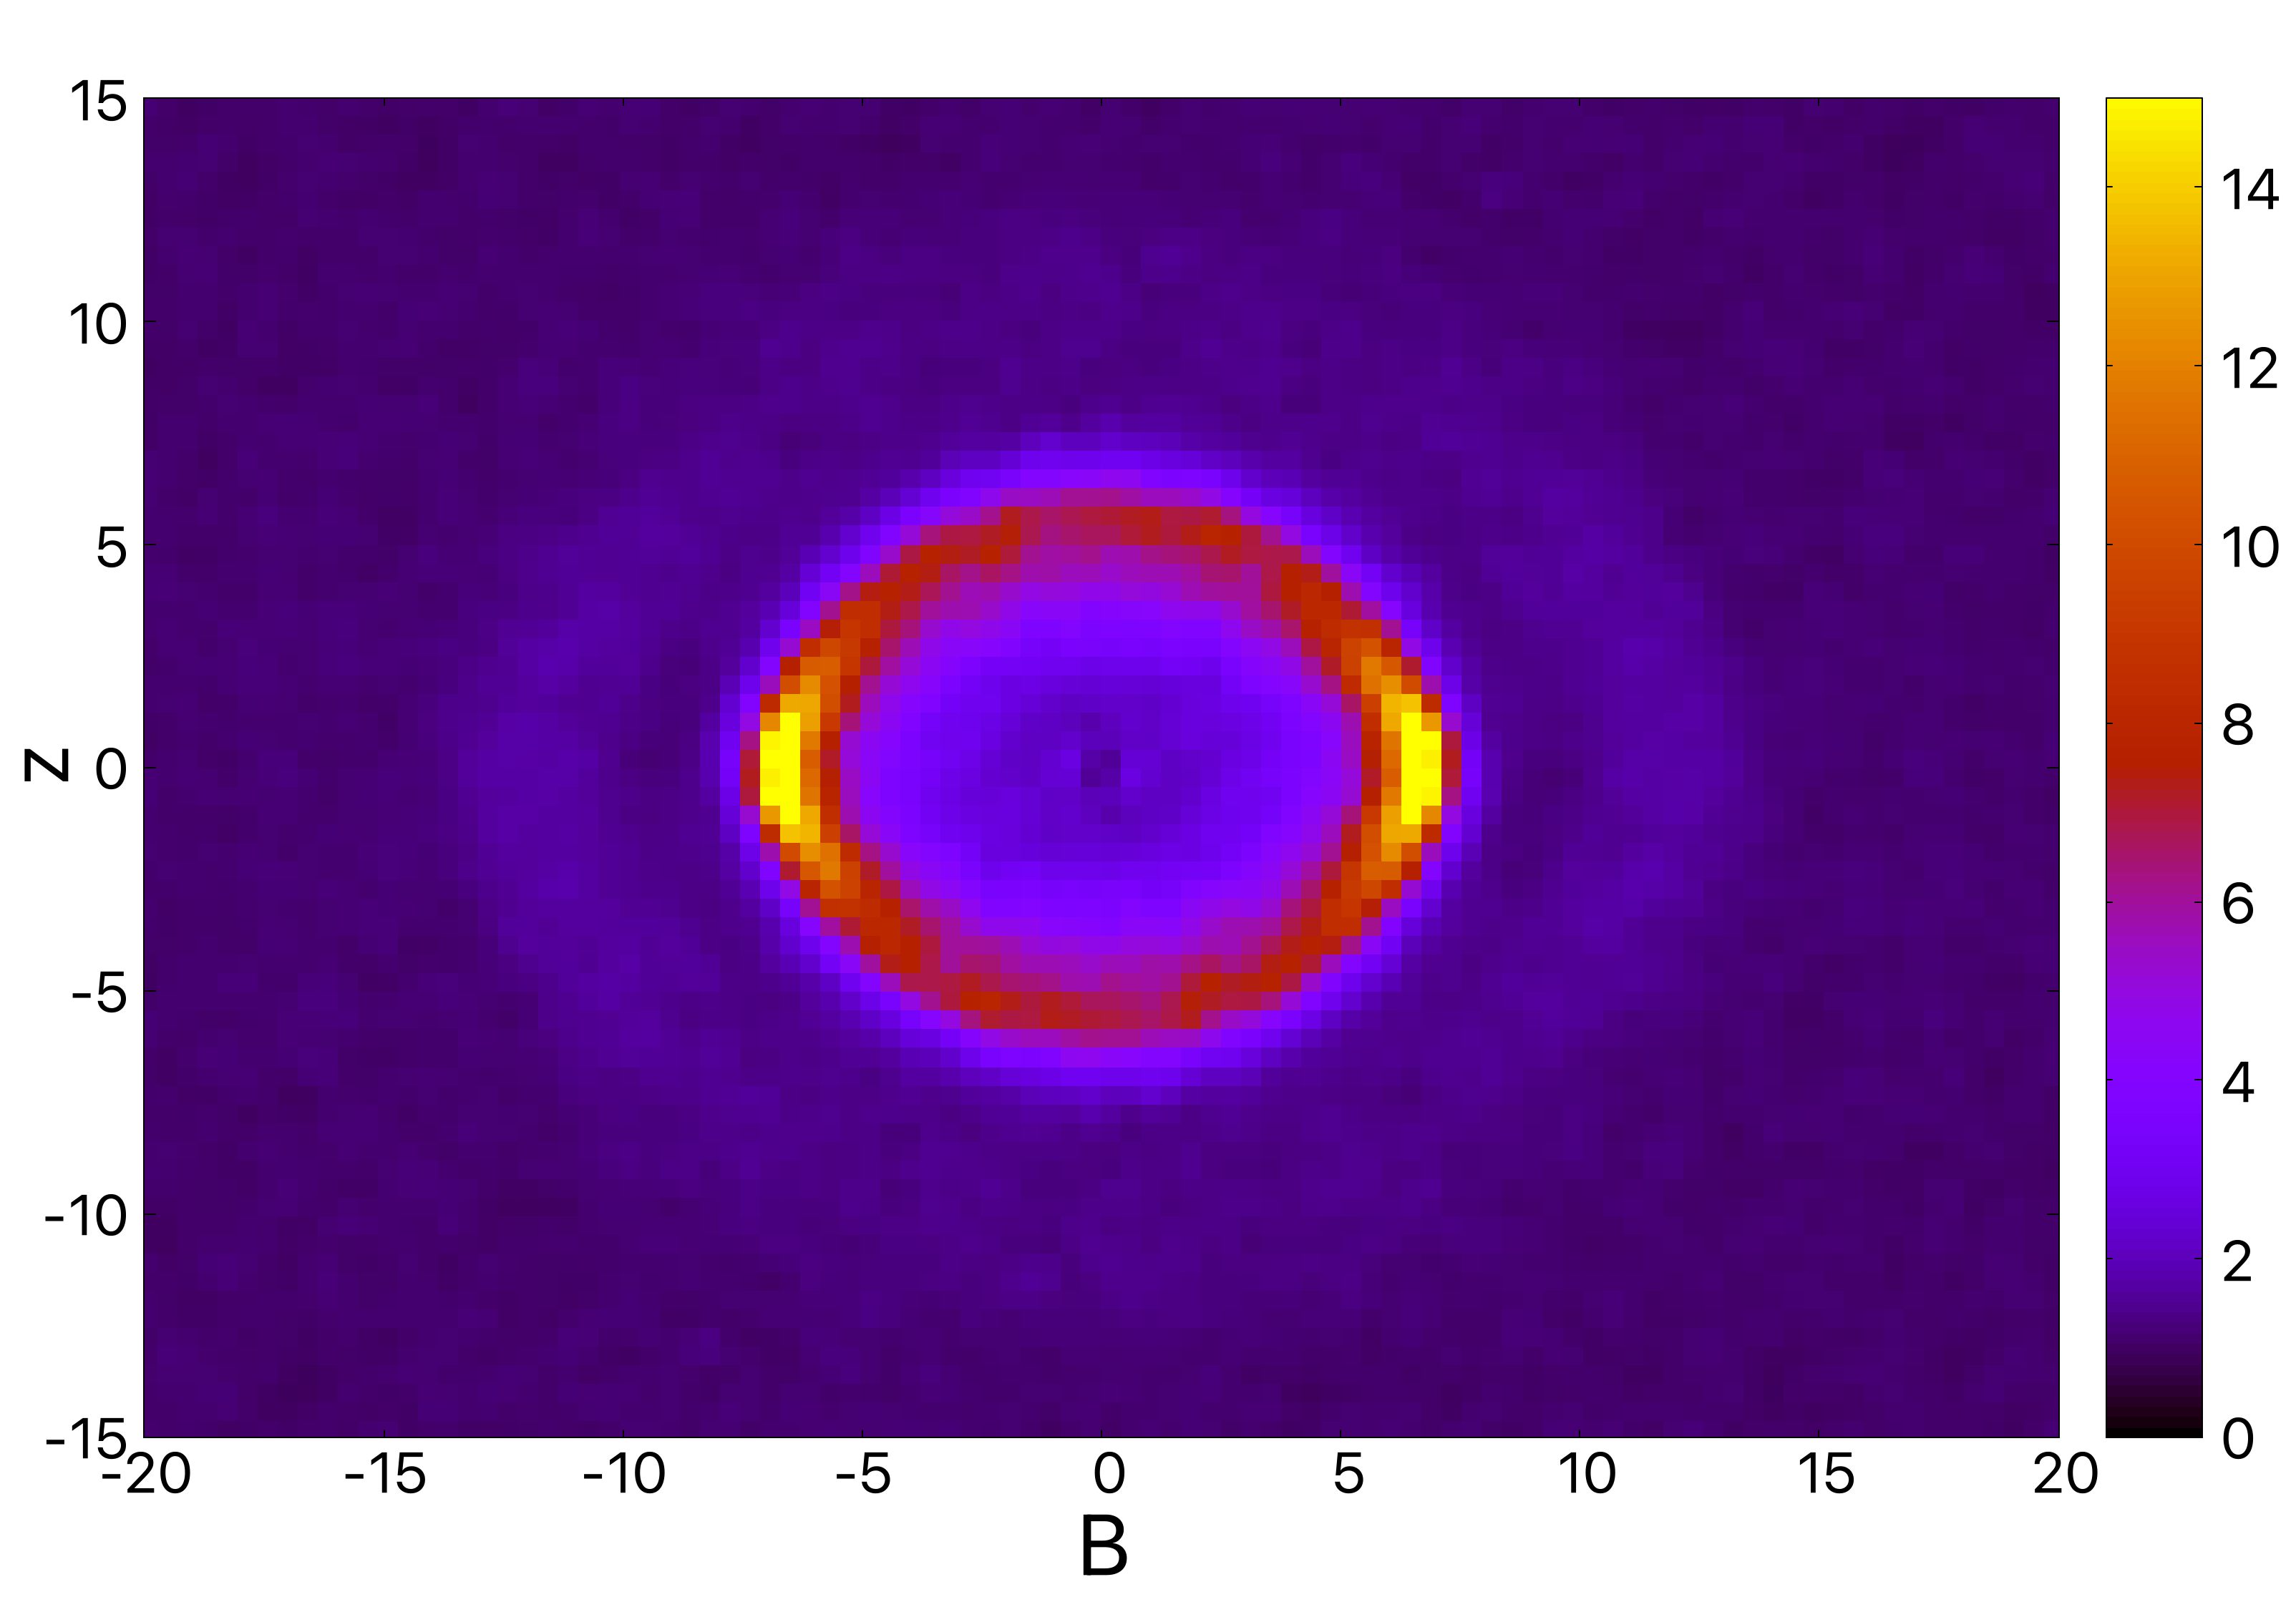
\includegraphics[width=0.5\columnwidth]{Syz_B_HE.png}
    \caption{Structure factor $S(0, q_y, q_z)$ of a system of HEs with a magnetic field along the y (B) axis at $\phi=0.50$.}\label{fig:Syz_B_HE}
\end{figure}

\begin{figure}
    \centering
    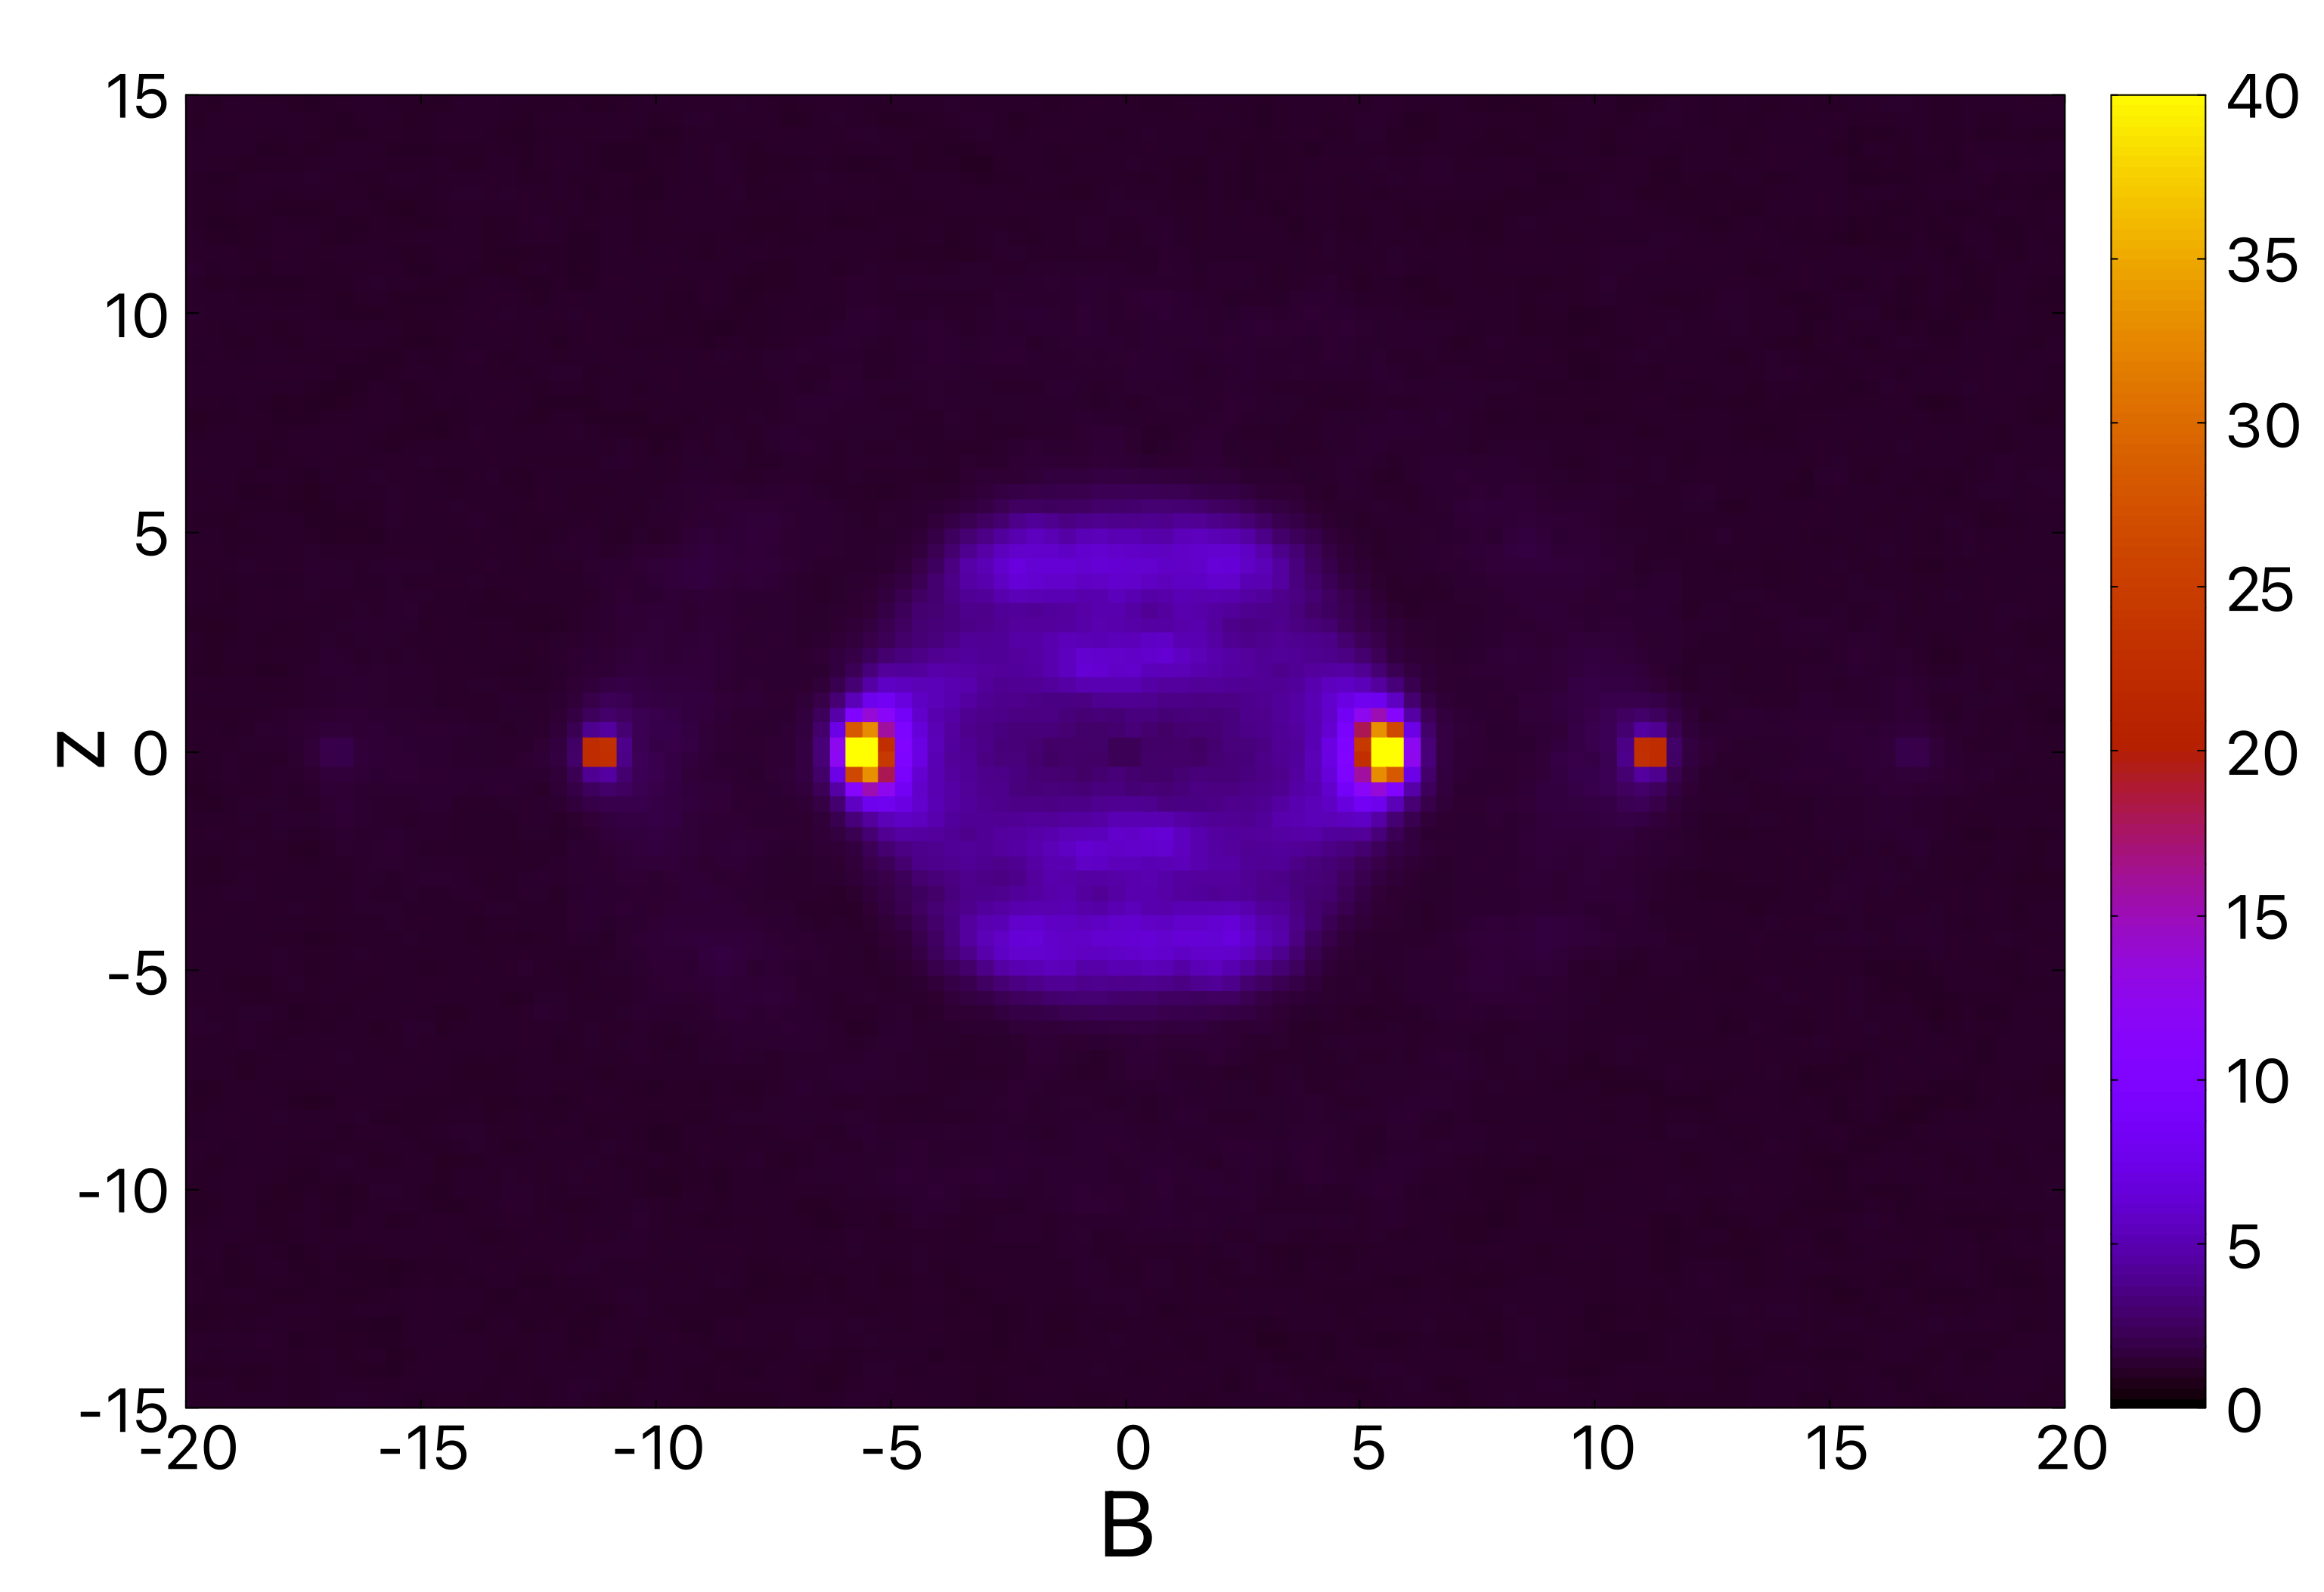
\includegraphics[width=0.5\columnwidth]{Syz_B.png}
    \caption{Structure factor $S(0, q_y, q_z)$ of a system of HSCs with a magnetic field along the y axis at $\phi=0.50$.}\label{fig:Syz_B_HSC}
\end{figure}

A way to characterize the smectic phase obtained from the simulations is provided by the calculation of the static structure factor~\cite{Hansen_McDonald}:

\begin{equation}\label{eq:S_q}
    S( \vec{q} ) = \left\langle \frac{1}{N} \rho_{\vec{q}} \rho_{-\vec{q}} \right\rangle 
\end{equation}

where $N$ is the number of scattering points, $\langle\ldots\rangle$ is an average over independent configurations and
$\rho_{\vec{q}}$ is the Fourier transform of the microscopic density:

\begin{equation}
    \rho_{\vec{q}} = \sum_{i=1}^N \exp(-i\, \vec{q} \cdot \vec{r}_i)
\end{equation}

Monte Carlo simulation in the NVT ensemble for both hard ellipsoids (HEs) and hard spherocylinders (HSCs) have been carried-out 
starting from a configuration at $\phi = 0.50$.
From these simulations we obtained many independent configurations for the centers of mass of both HEs and HSCs. 
In these configurations we replaced each particle with a set of scattering points randomly placed inside it and 
of fixed number density, as shown in Figs.~\ref{fig:scatt_mod_single} and~\ref{fig:scatt_mod1}. 
Finally, by using these random sets of points in Eq.~\ref{eq:S_q} we calculated the static structure factor $S(q)$ 
onto the plane $yz$ parallel to the magnetic field (i.e.~we calculated $S(0, q_y, q_z)$), where, here and in the following,
the y-axis is assumed to be parallel to the external magnetic field.
The results are shown in Fig.~\ref{fig:Syz_B_HE} for HEs and in Fig.~\ref{fig:Syz_B_HSC} for HSCs.

\subsection{Pair distribution function}

The phase behavior can be also characterized by calculating the three-dimensional pair distribution function $g(\vec{r})$, i.e.:

\begin{equation}
    g(\vec{r}) = \frac{1}{\rho N} \left\langle \sum_{i=1}^N \sum_{j\neq i} \delta \left( \vec{r} - \left( \vec{r}_i - \vec{r}_j \right) \right) \right\rangle
\end{equation}

where $\delta(x)$ is the Dirac delta function and $\langle\ldots\rangle$ is an average over independent configurations.
We calculated the $g(\vec{r})$ onto the planes $yz$ and $xz$, which are parallel and perpendicular to the magnetic field, respectively. 
The results are shown in Fig.~\ref{fig:gyz_B} and Fig.~\ref{fig:gxz_B} from which the smectic ordering is rather apparent.
Differently, the radial distribution function of HEs does not show any
layering for all state points studies. A typical example of $g(r)$ for HEs is shown in Fig.~\ref{fig:gyz_B_HE} (yz-plane) and 
Fig.~\ref{fig:gxz_B_HE} (xz-plane). The anisotropy and structuring shown in Fig.~\ref{fig:gyz_B_HE} reflects the alignment 
of HEs due to the magnetic field. Differently, the anisotropy
of the radial distribution function calculated onto a plane perpendicular to the magnetic field, which is shown in 
Fig.~\ref{fig:gxz_B_HE}, is due to orientational ordering of HEs, which builds up at volume fractions higher than $\approx 0.45$.  
More details on this are provided below (see subsection I-D entitled ``Smectic and nematic order parameters'').

\begin{figure}
    \begin{center}
    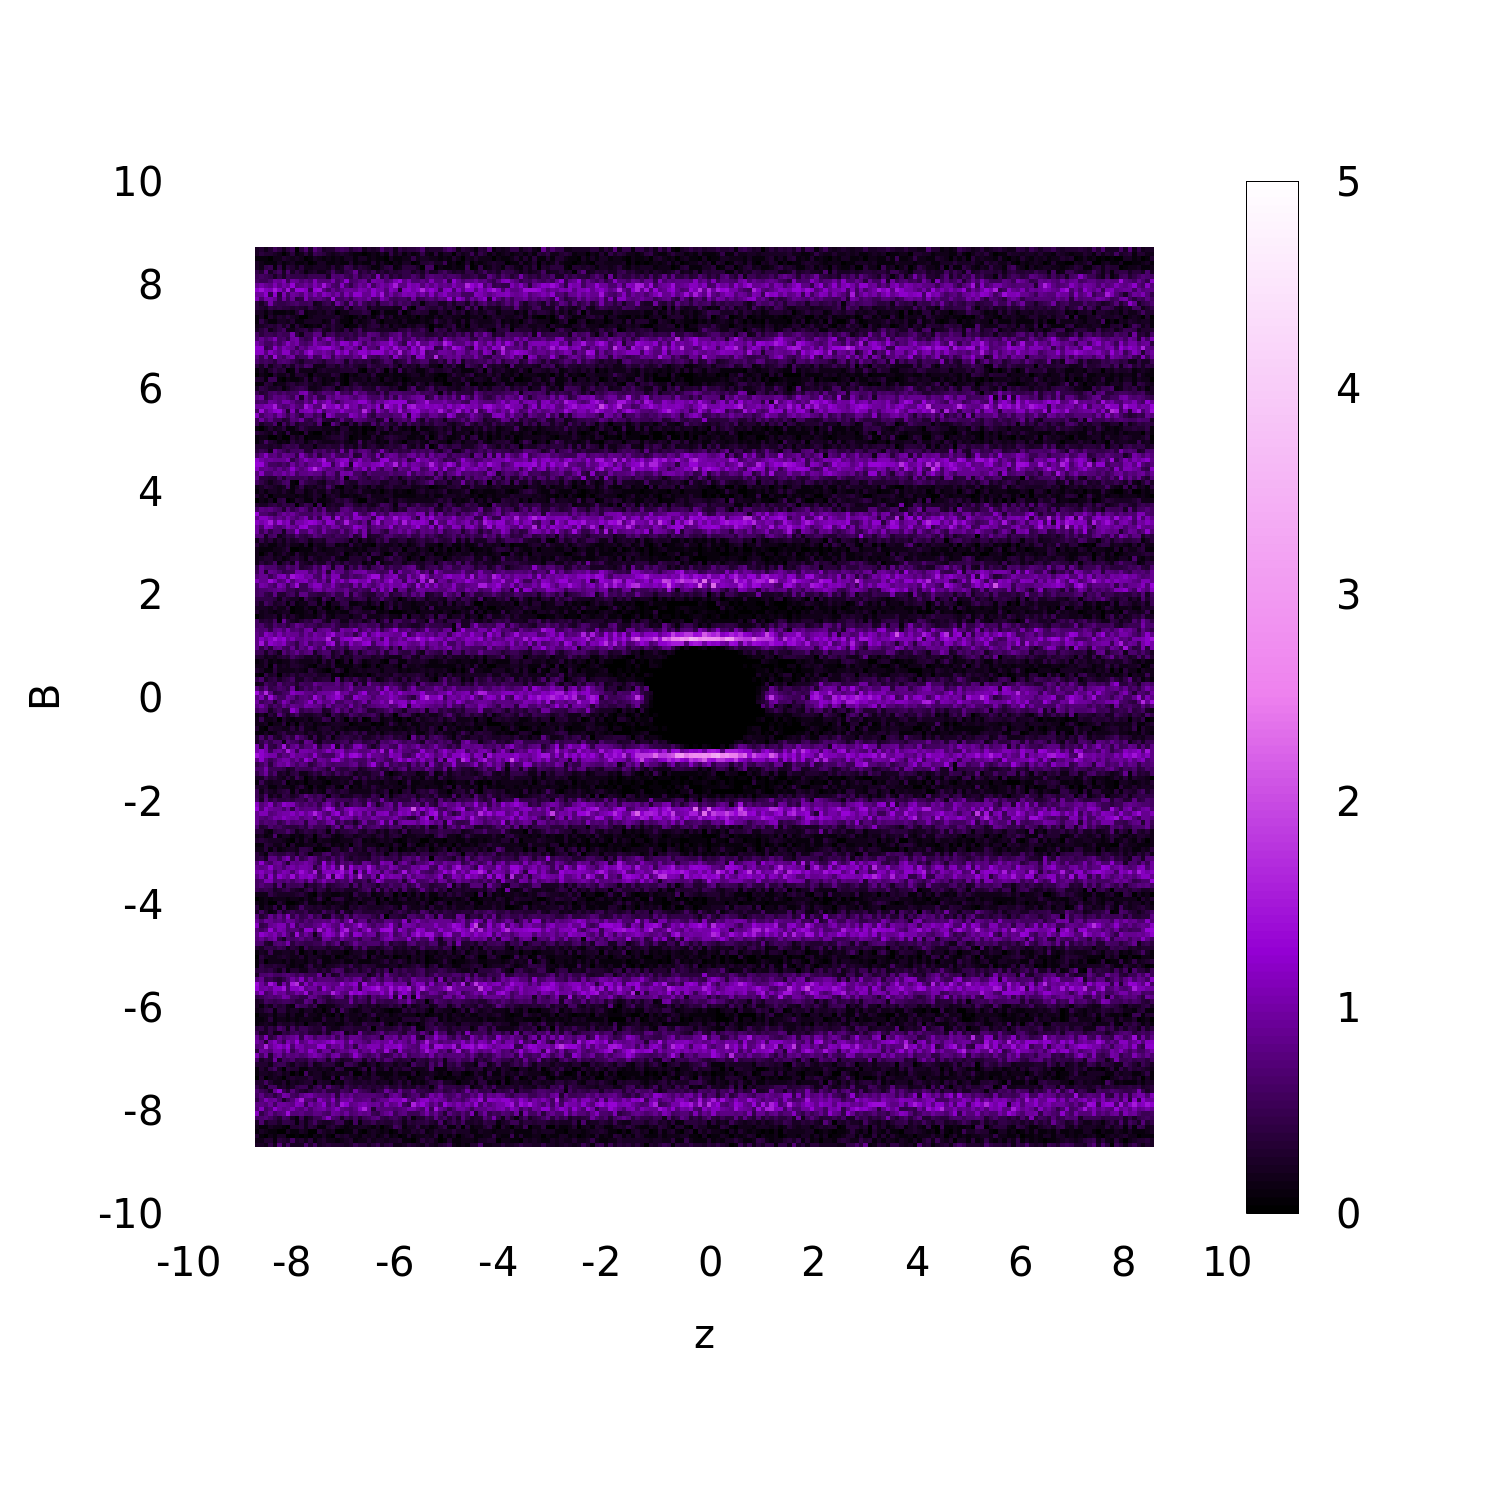
\includegraphics[width=0.5\columnwidth]{gyz_B.png}
    \caption{Pair distribution function for a system of HSCs $\phi = 0.50$ with a magnetic field $\vec{B}$ directed along y axis.}\label{fig:gyz_B}
    \end{center}
\end{figure}


\begin{figure}
    \centering
    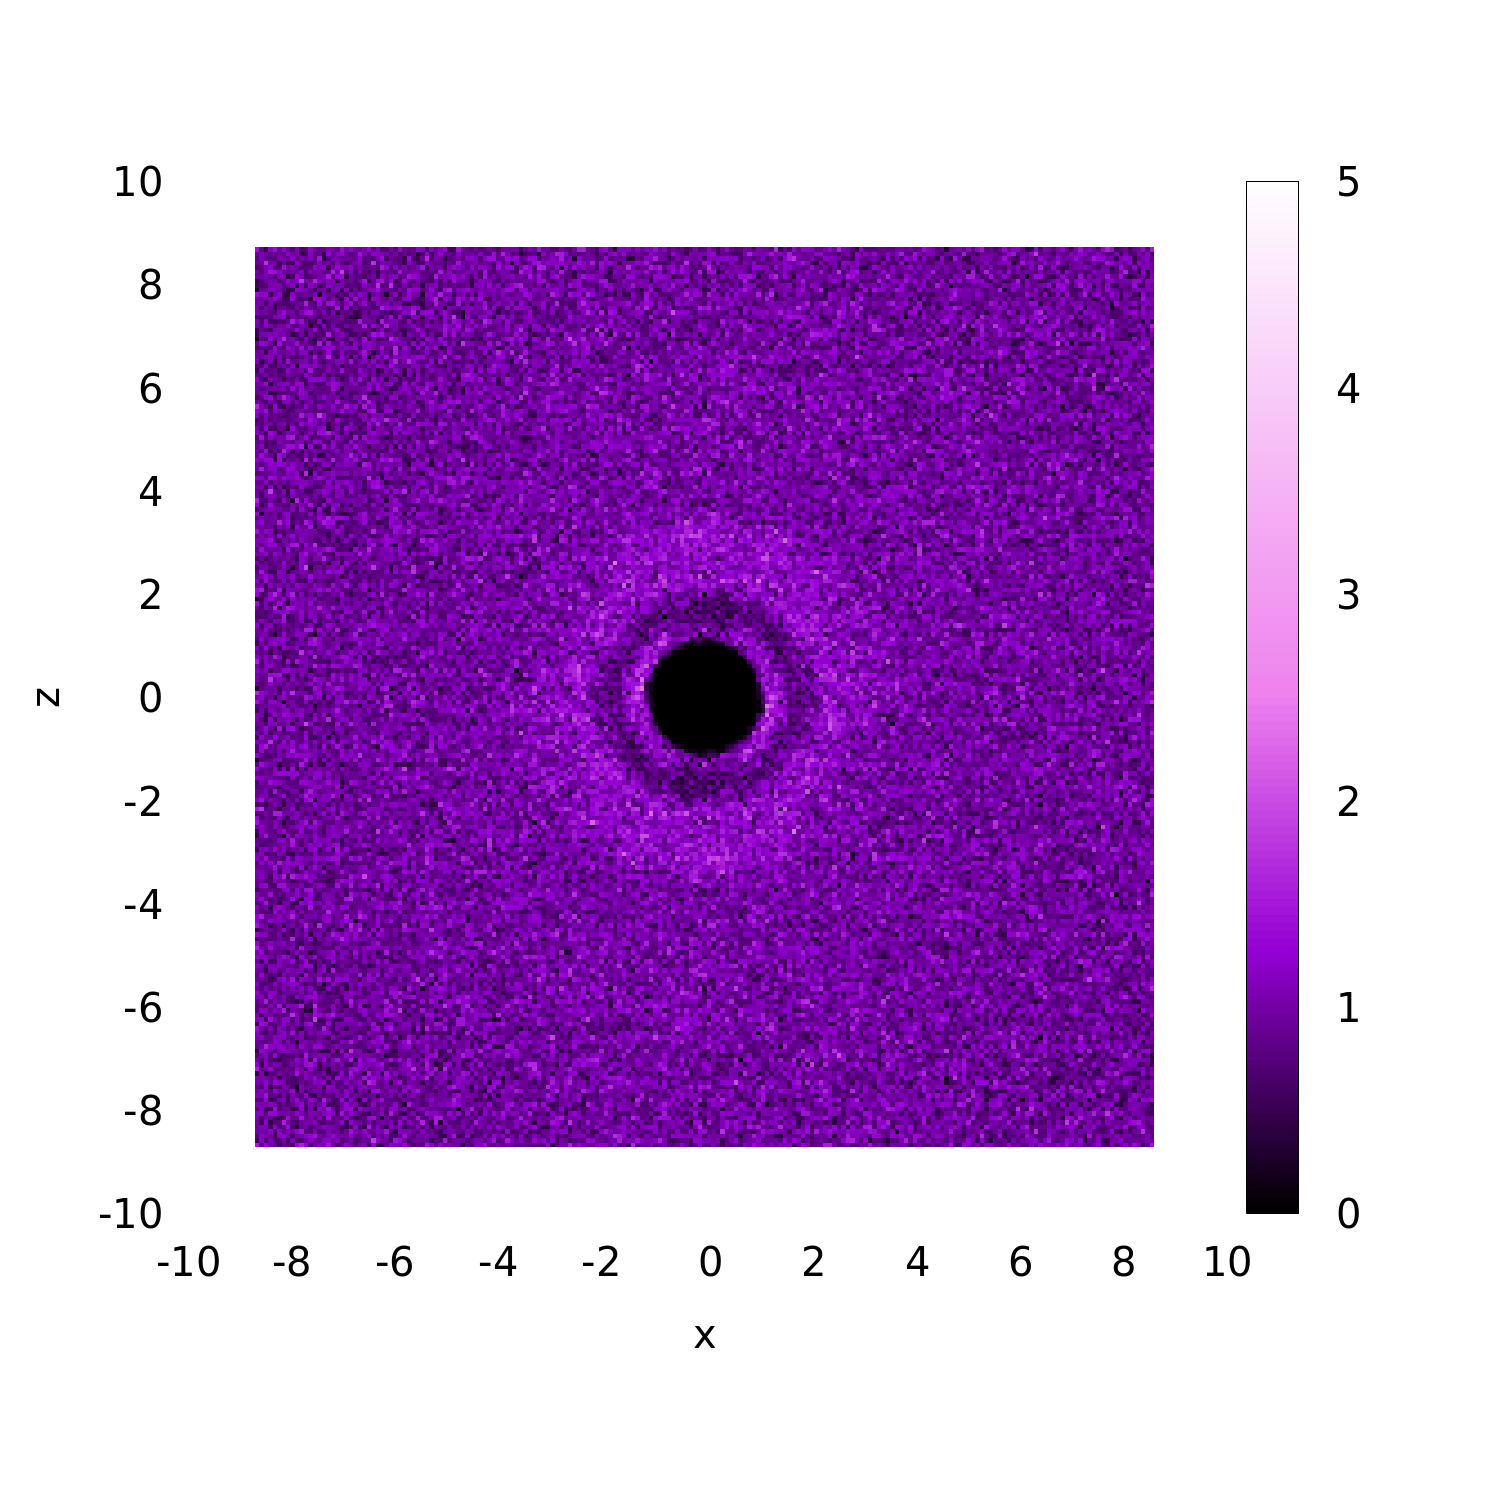
\includegraphics[width=0.5\columnwidth]{gxz_B.png}
    \caption{Pair distribution function for a system of HSCs $\phi = 0.50$ with a magnetic field $\vec{B}$ directed along the y-axis.}\label{fig:gxz_B}
\end{figure}

\begin{figure}
    \begin{center}
    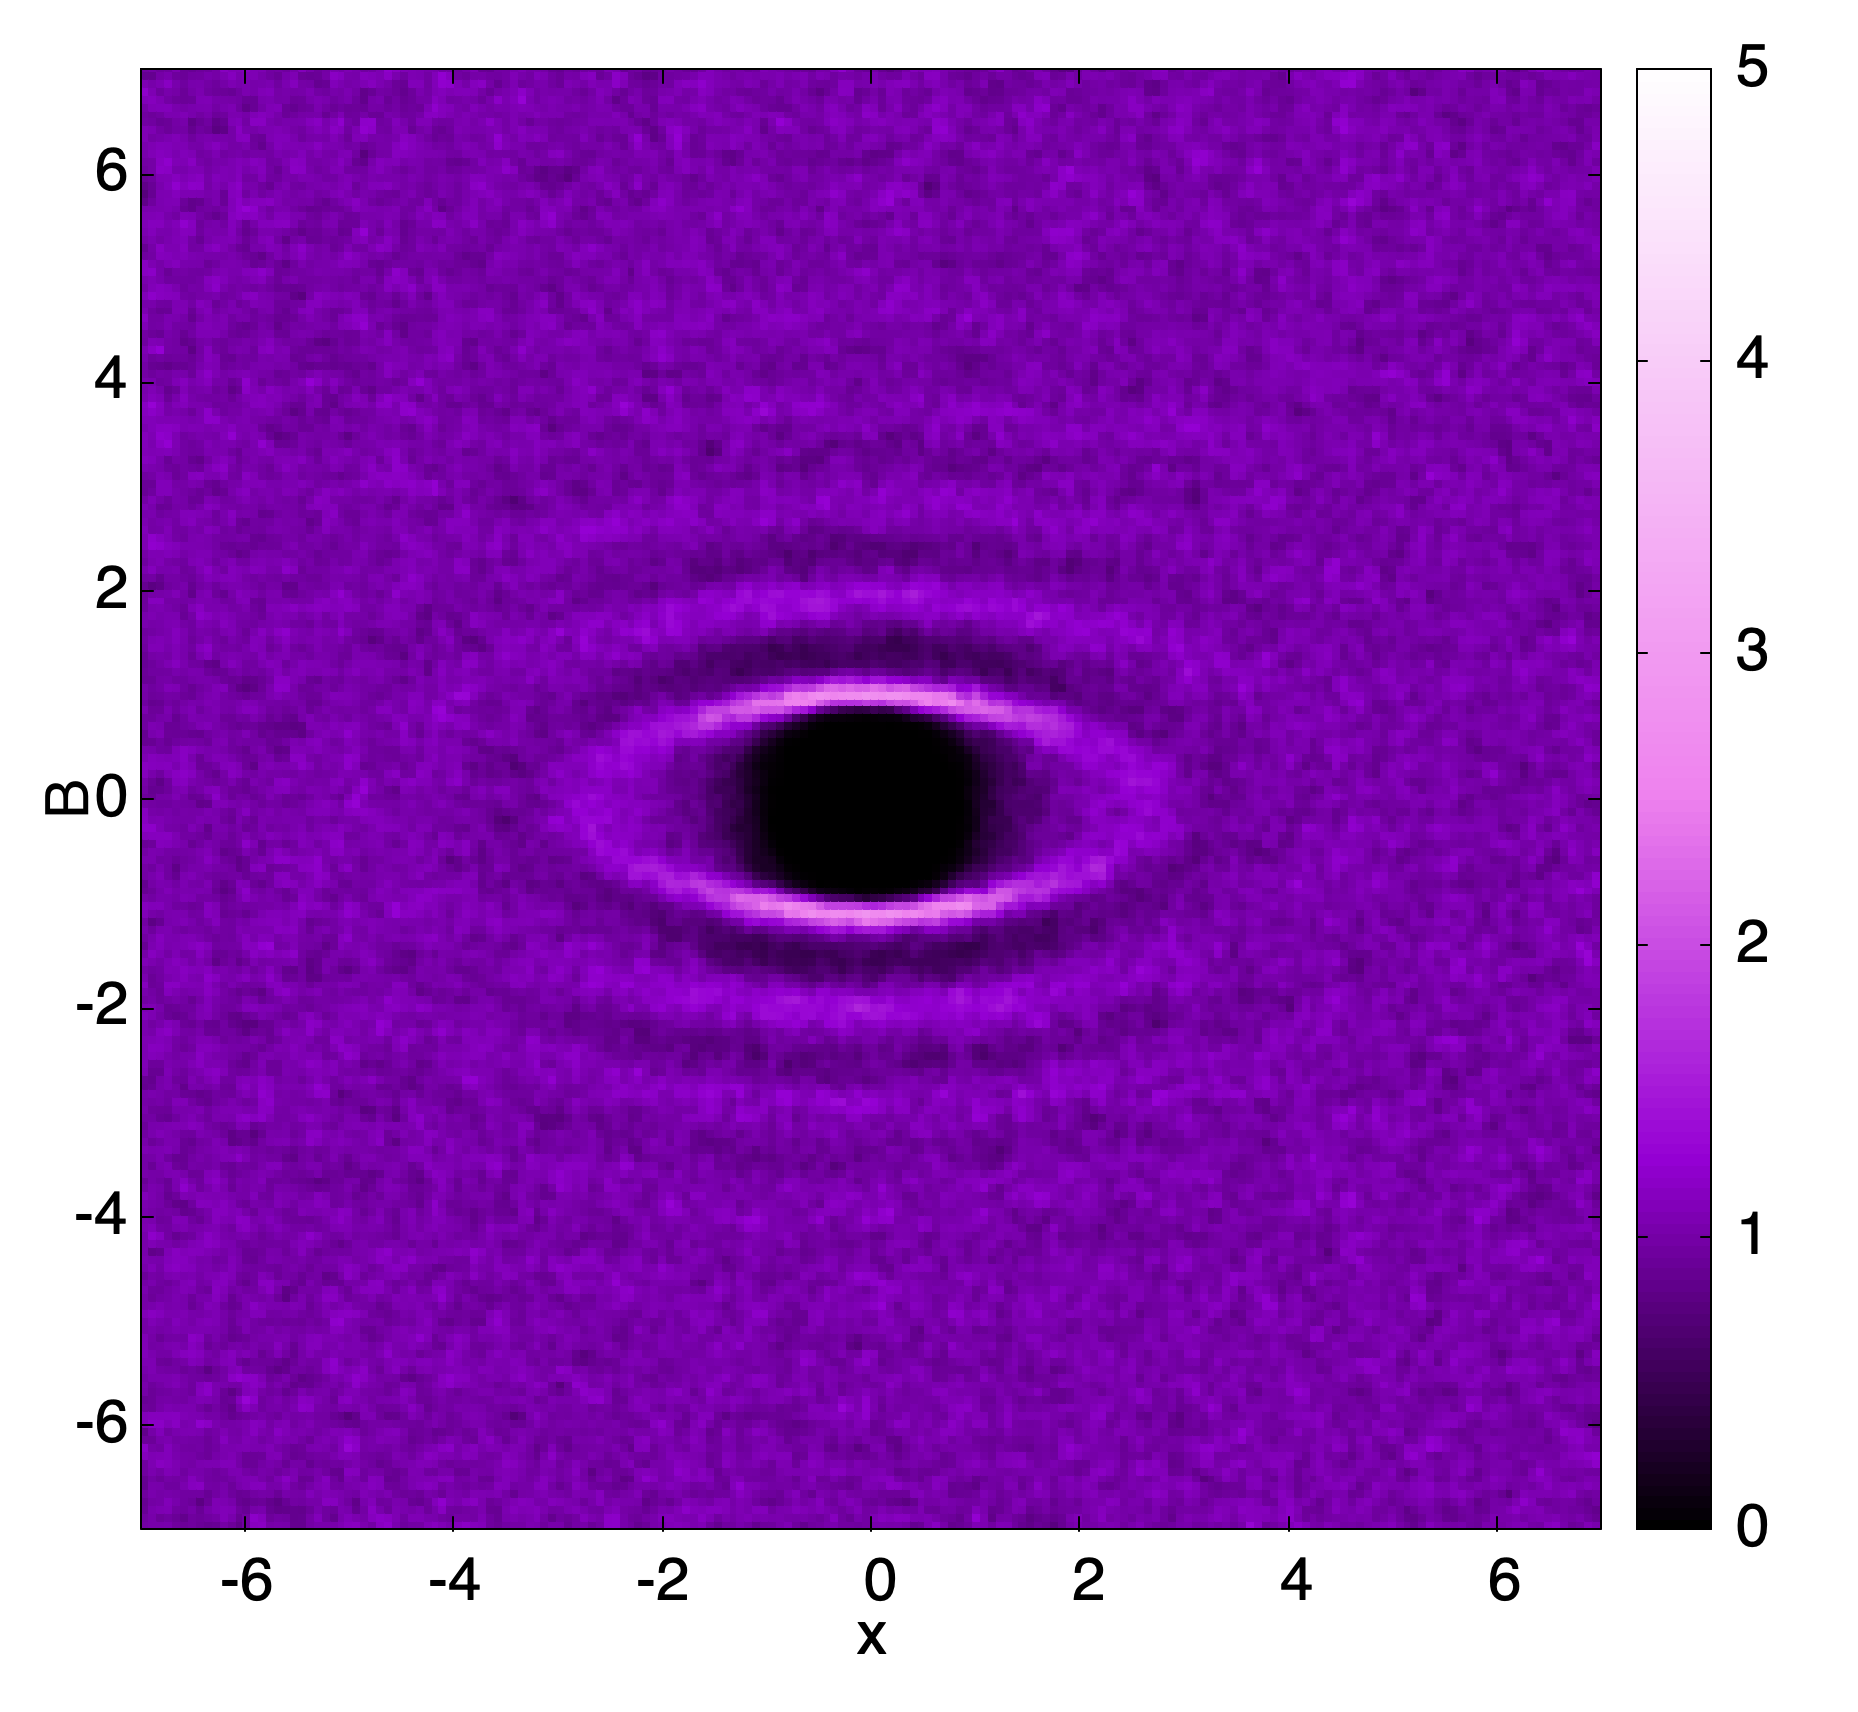
\includegraphics[width=0.4\columnwidth]{gyz_B_HE.png}
    \caption{Pair distribution function for a system of HEs at $\phi = 0.50$ with a magnetic field $\vec{B}$ directed along the y-axis.}\label{fig:gyz_B_HE}
    \end{center}
\end{figure}


\begin{figure}
    \centering
    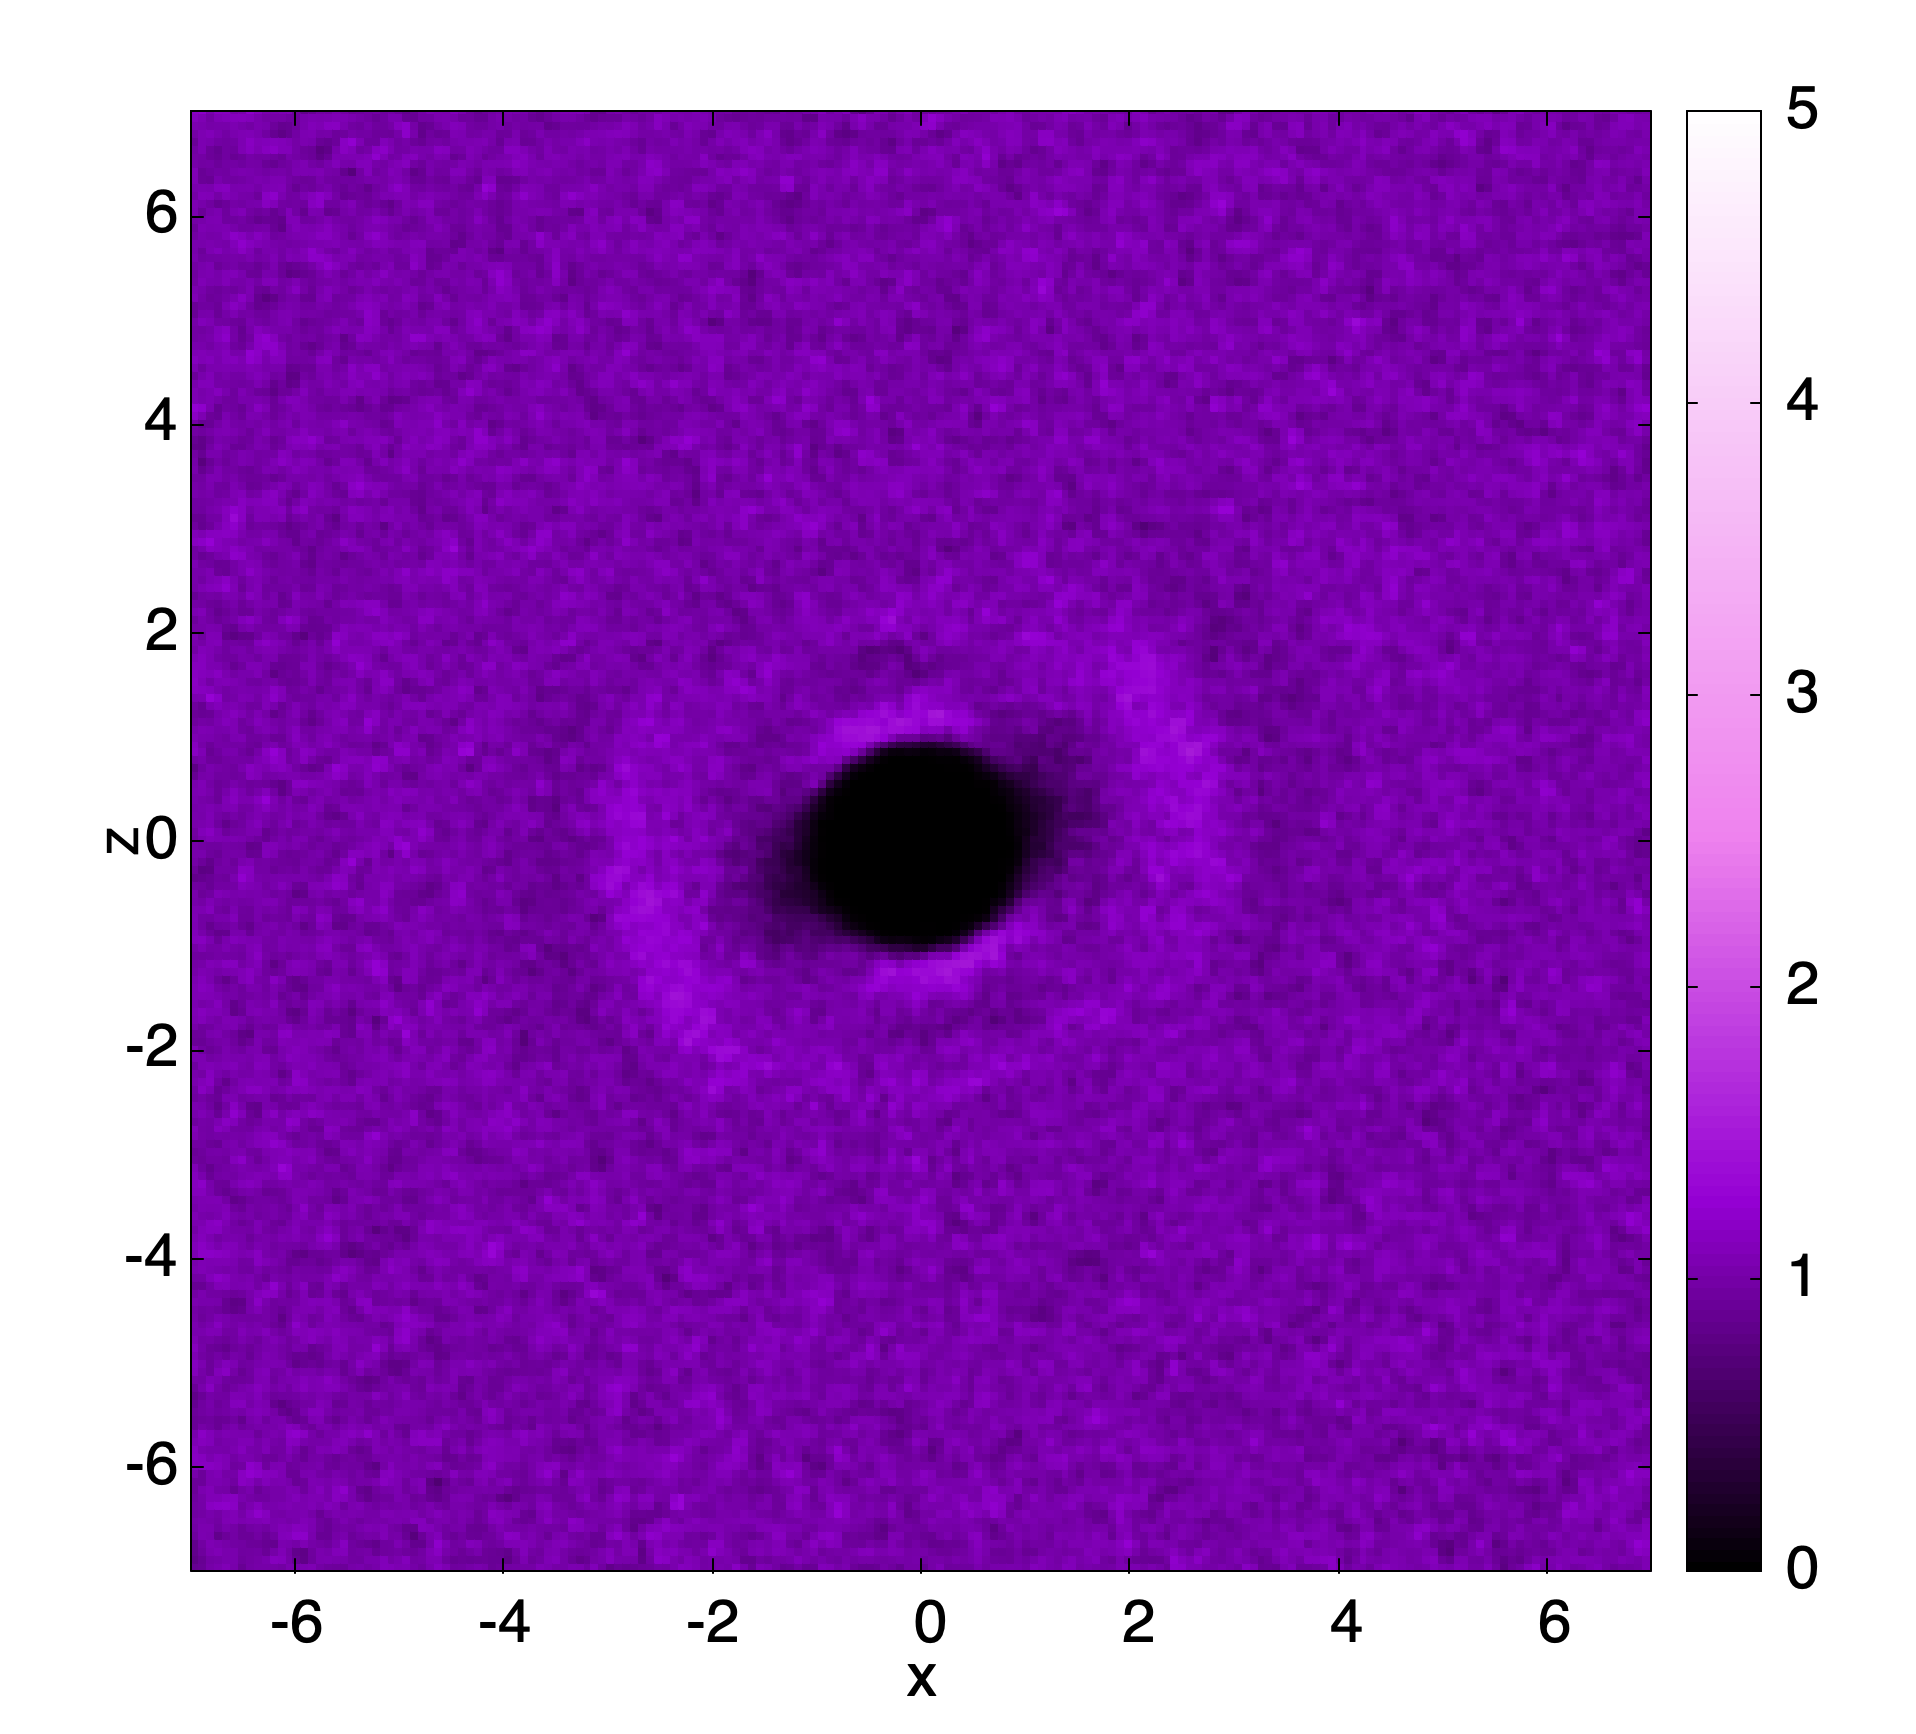
\includegraphics[width=0.4\columnwidth]{gxz_B_HE.png}
    \caption{Pair distribution function for a system of HEs at $\phi = 0.50$ with a magnetic field $\vec{B}$ along the y-axis.}\label{fig:gxz_B_HE}
\end{figure}
%\newpage %usato solo per non far andare l'immagine prima

\subsection{Smectic and nematic order parameters}

A convenient way to check the emergence of a smectic phase in our computer simulations 
is to calculate the smectic order parameter $\tau_1$ defined as follows:

\begin{equation}
    \tau_1 = \langle | \sum_i e^{i 2\pi \vec{r}_i \cdot \hat{n} / d } |\rangle 
\end{equation}

where $\langle\ldots\rangle$ is an average over several independent configurations, $\vec{r}_i$ is the position of the $i$-th particle, $\hat{n}$ is the direction of the magnetic
field and $d$ is the thickness of the smectic layers.
In order to compute $\tau_1$ for each configuration we find the optimal value of $d$, i.e. 
the value which maximizes $\tau_1$.

The values of $\tau_1$ for both HSCs and HEs and for all pressures studied is shown in Fig.~\ref{fig:ordpars} (top). It can be seen that HSCs exhibit a range of volume fractions where 
a smectic layer ordering is present and which coincide with the green state points shown in Fig. 7(a)
in the main test. On the contrary no evidence of layering emerges in the simulation of HEs.

\begin{figure}
    \centering
    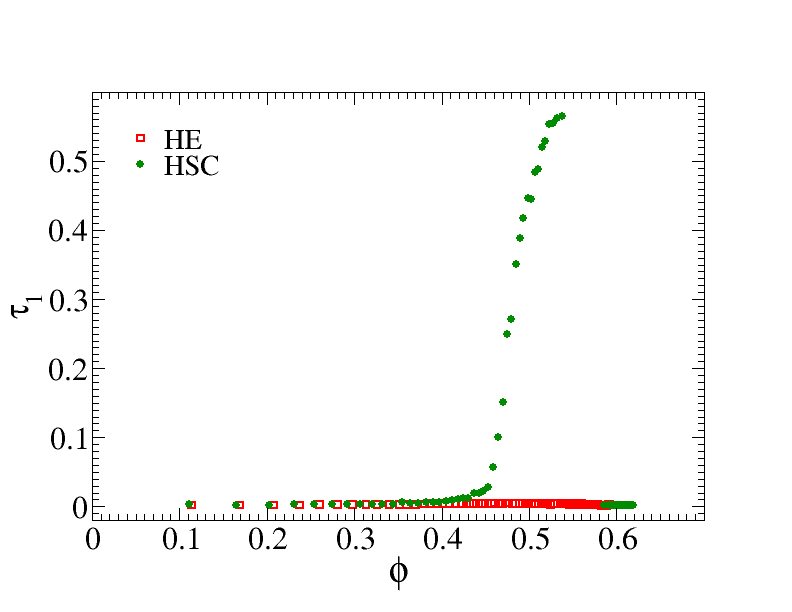
\includegraphics[width=0.45\columnwidth]{smordpar.png}
    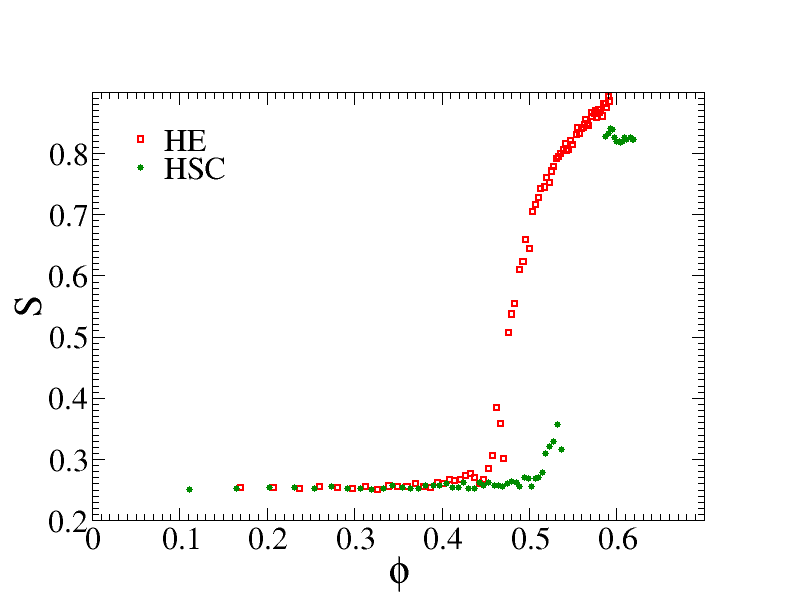
\includegraphics[width=0.45\columnwidth]{nemop.png}  
    \caption{Smectic ($\tau_1$, top) and nematic ($S$, bottom) order parameters for HSCs and HEs.}\label{fig:ordpars}
\end{figure}

We also calculated the nematic order parameter $S$ related to the symmetry axis of HSC and HE, which
is defined as the largest eigenvalue of the order tensor $Q$, whose components are:
\begin{equation}
  Q_{\alpha\beta} = \frac{1}{N} \sum_i \frac{3}{2} \langle {(\vec{u}_i)}_\alpha {(\vec{u}_i)}_\beta\rangle
\label{eq:nemop}
\end{equation}
where $\alpha\beta\in\{x,y,z\}$ and the unit vector ${(\mathbf{u}_i)}_\alpha$ is the component $\alpha$ of the orientation (i.e.~the symmetry axis) of particle $i$.
First we note that since particles are aligned perpendicularly to the nematic field, if they are 
randomly oriented one has $S=1/4$. Hence, below $\phi_0 < 0.45$ both symmetry axis of HSC and HE are 
randomly oriented onto the plance perpendicular to the magnetic field.
Interestingly, for $\phi > \phi_0$ HSC starts exhibiting smectic layering but their orientations
remain random, while orientations of HE starts aligning (see Fig.~\ref{fig:ordpars} (bottom)).


\section{Simulations without magnetic field}

In order to demonstrate that the smectic phase observed in the simulations of HSCs is induced by the external magnetic field, 
we performed a NTV Monte Carlo simulation without the external magnetic field at $\phi=0.50$ starting from a smectic configuration  
of HSCs.  As shown in Fig.~\ref{fig:noB_snapshot}, the system is isotropic, 
thus proving that the smectic phase is an exquisite filed-induced effect.

\subsection{Structure factor}
To verify that by switching-off the external field an isotropic phase is obtained, 
we calculated also the static structure factor $S(0, q_y, q_z)$, which exhibits a typical isotropic pattern, 
as shown in Fig.~\ref{fig:Syz_noB}.

%\newpage    %da togliere

\begin{figure}
    \centering
    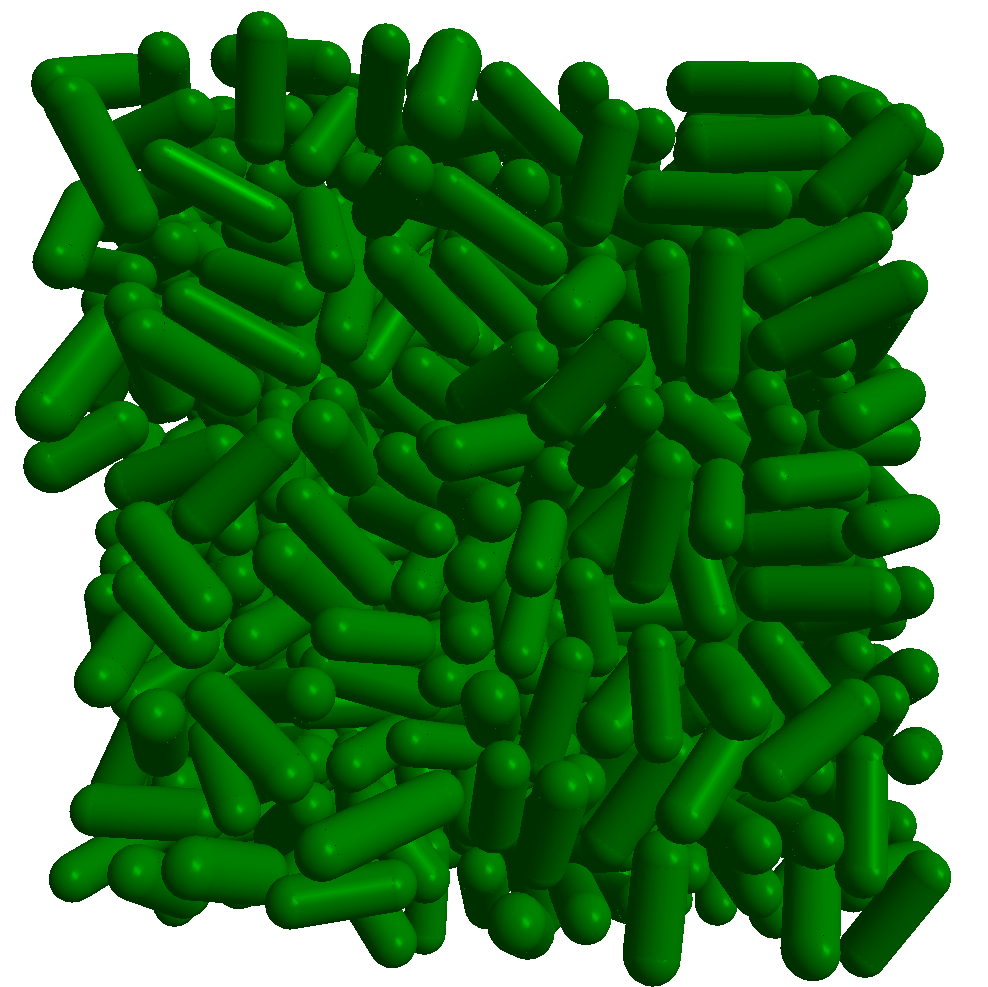
\includegraphics[width=0.4\columnwidth]{Isotropic_phase_snap.png}
    \caption{Snapshot of a system of HSCs with $\phi = 0.50$ without an external magnetic field.}\label{fig:noB_snapshot}
\end{figure}

\begin{figure}
    \centering
    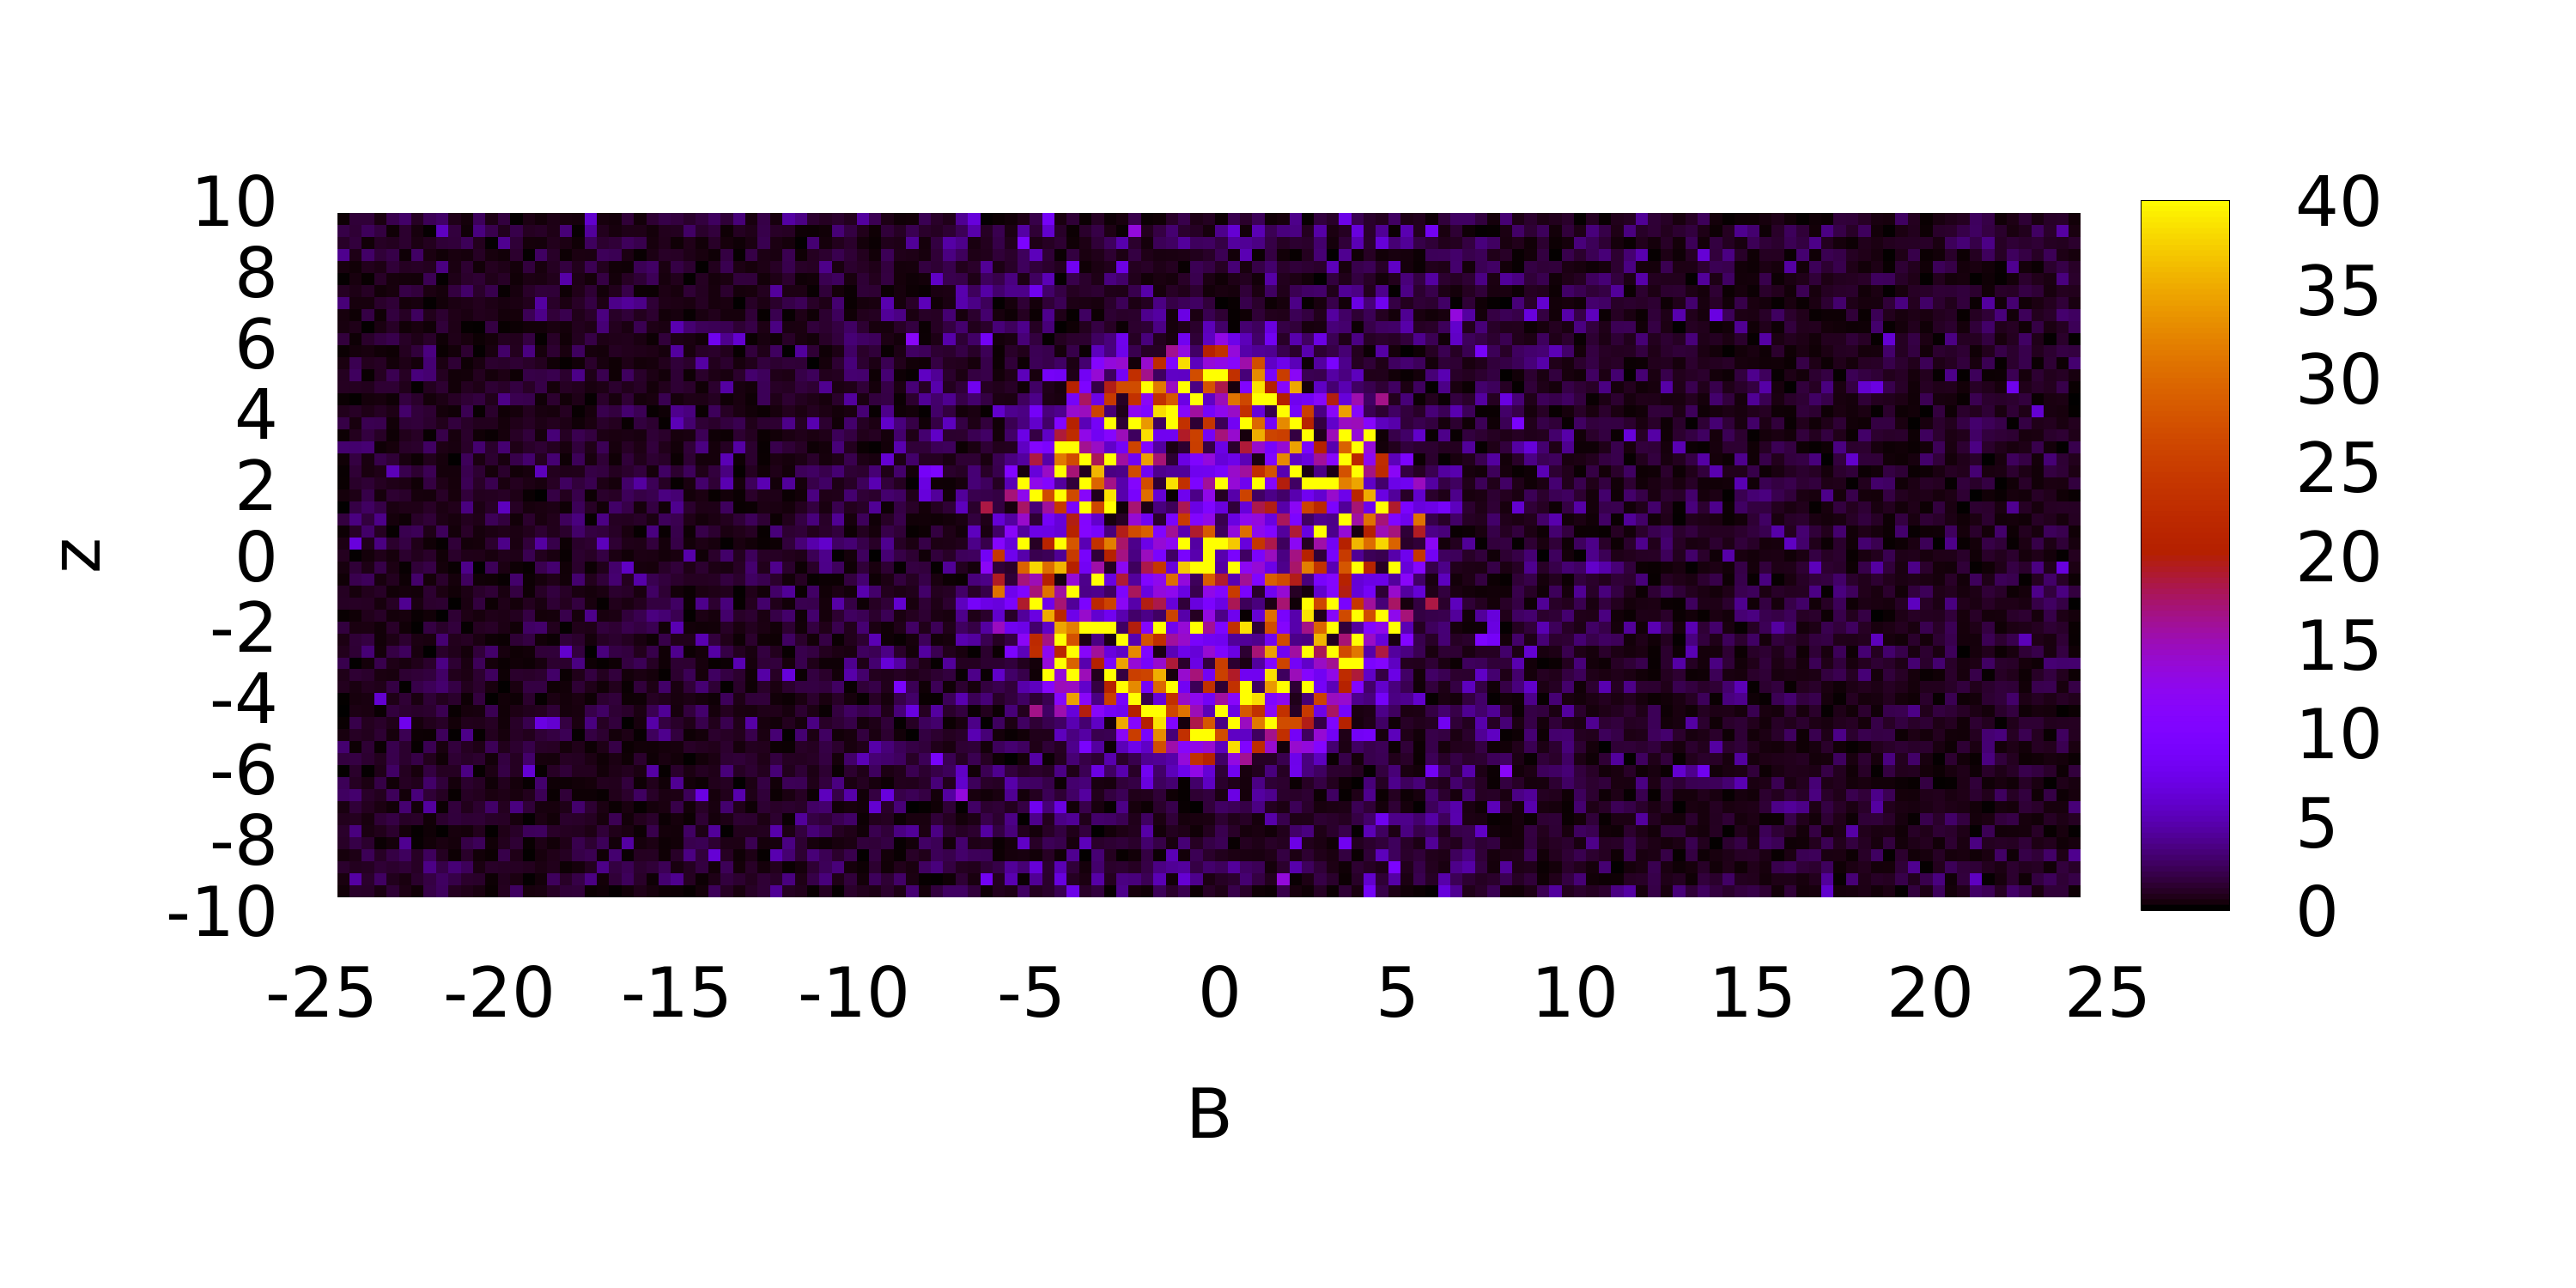
\includegraphics[width=0.7\columnwidth]{Syz_noB.png}
    \caption{Structure factor $S(0, q_y, q_z)$ of HSCs without a magnetic field at $\phi=0.50$.}\label{fig:Syz_noB}
\end{figure}

\subsection{Pair distribution function}

We also calculated the pair distribution function for HSCs with the magnetic field switched-off. 
As it can be seen in Figs.~\ref{fig:gxz_noB} and~\ref{fig:gyz_noB}, the system is isotropic, i.e.~long range
spatial correlation between the particles are absent, thus confirming the field-induced nature of the smectic phase.

\begin{figure}
    \centering
    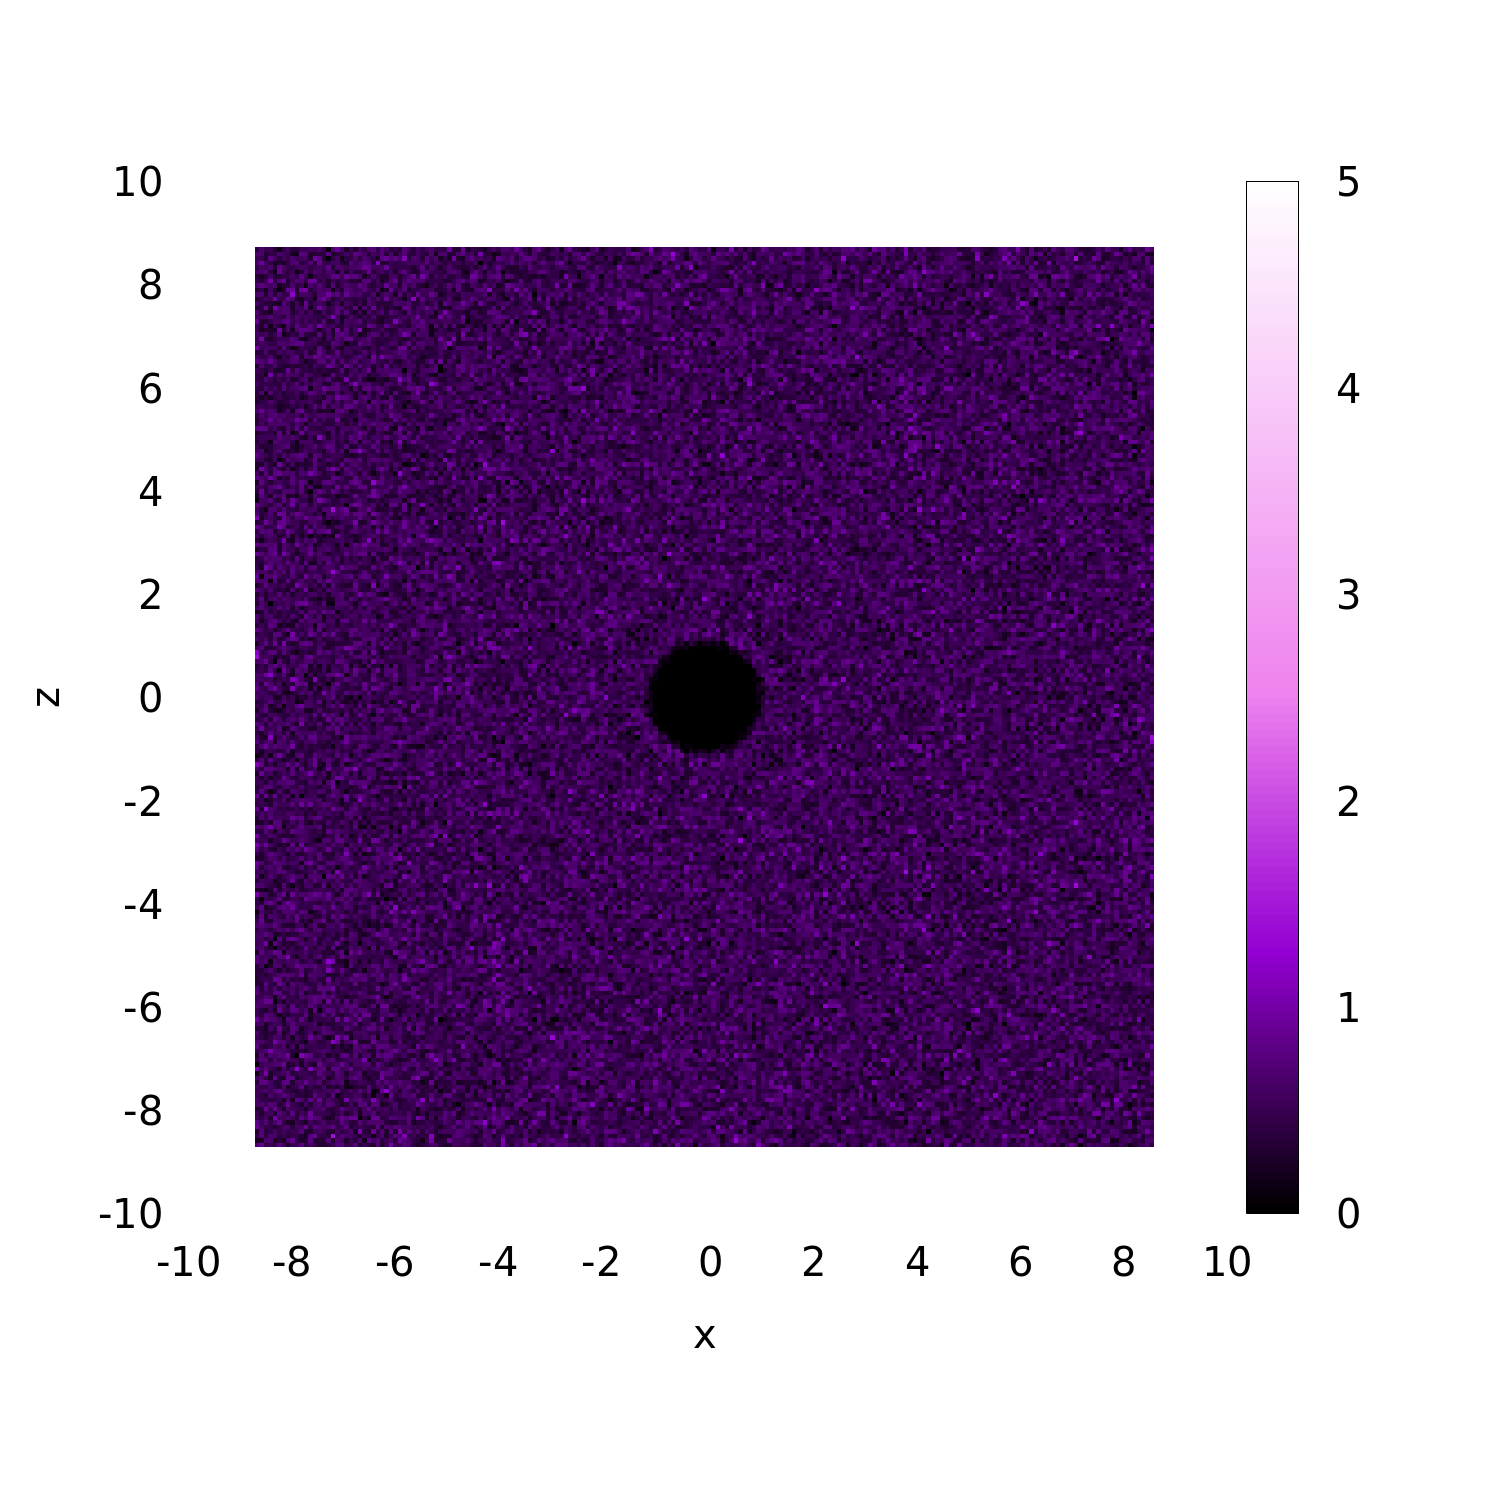
\includegraphics[width=0.5\columnwidth]{gxz_noB.png}
    \caption{Pair distribution function of HSCs without a magnetic field on the xz-plane at $\phi=0.50$.}\label{fig:gxz_noB}
\end{figure}

\begin{figure}
    \centering
    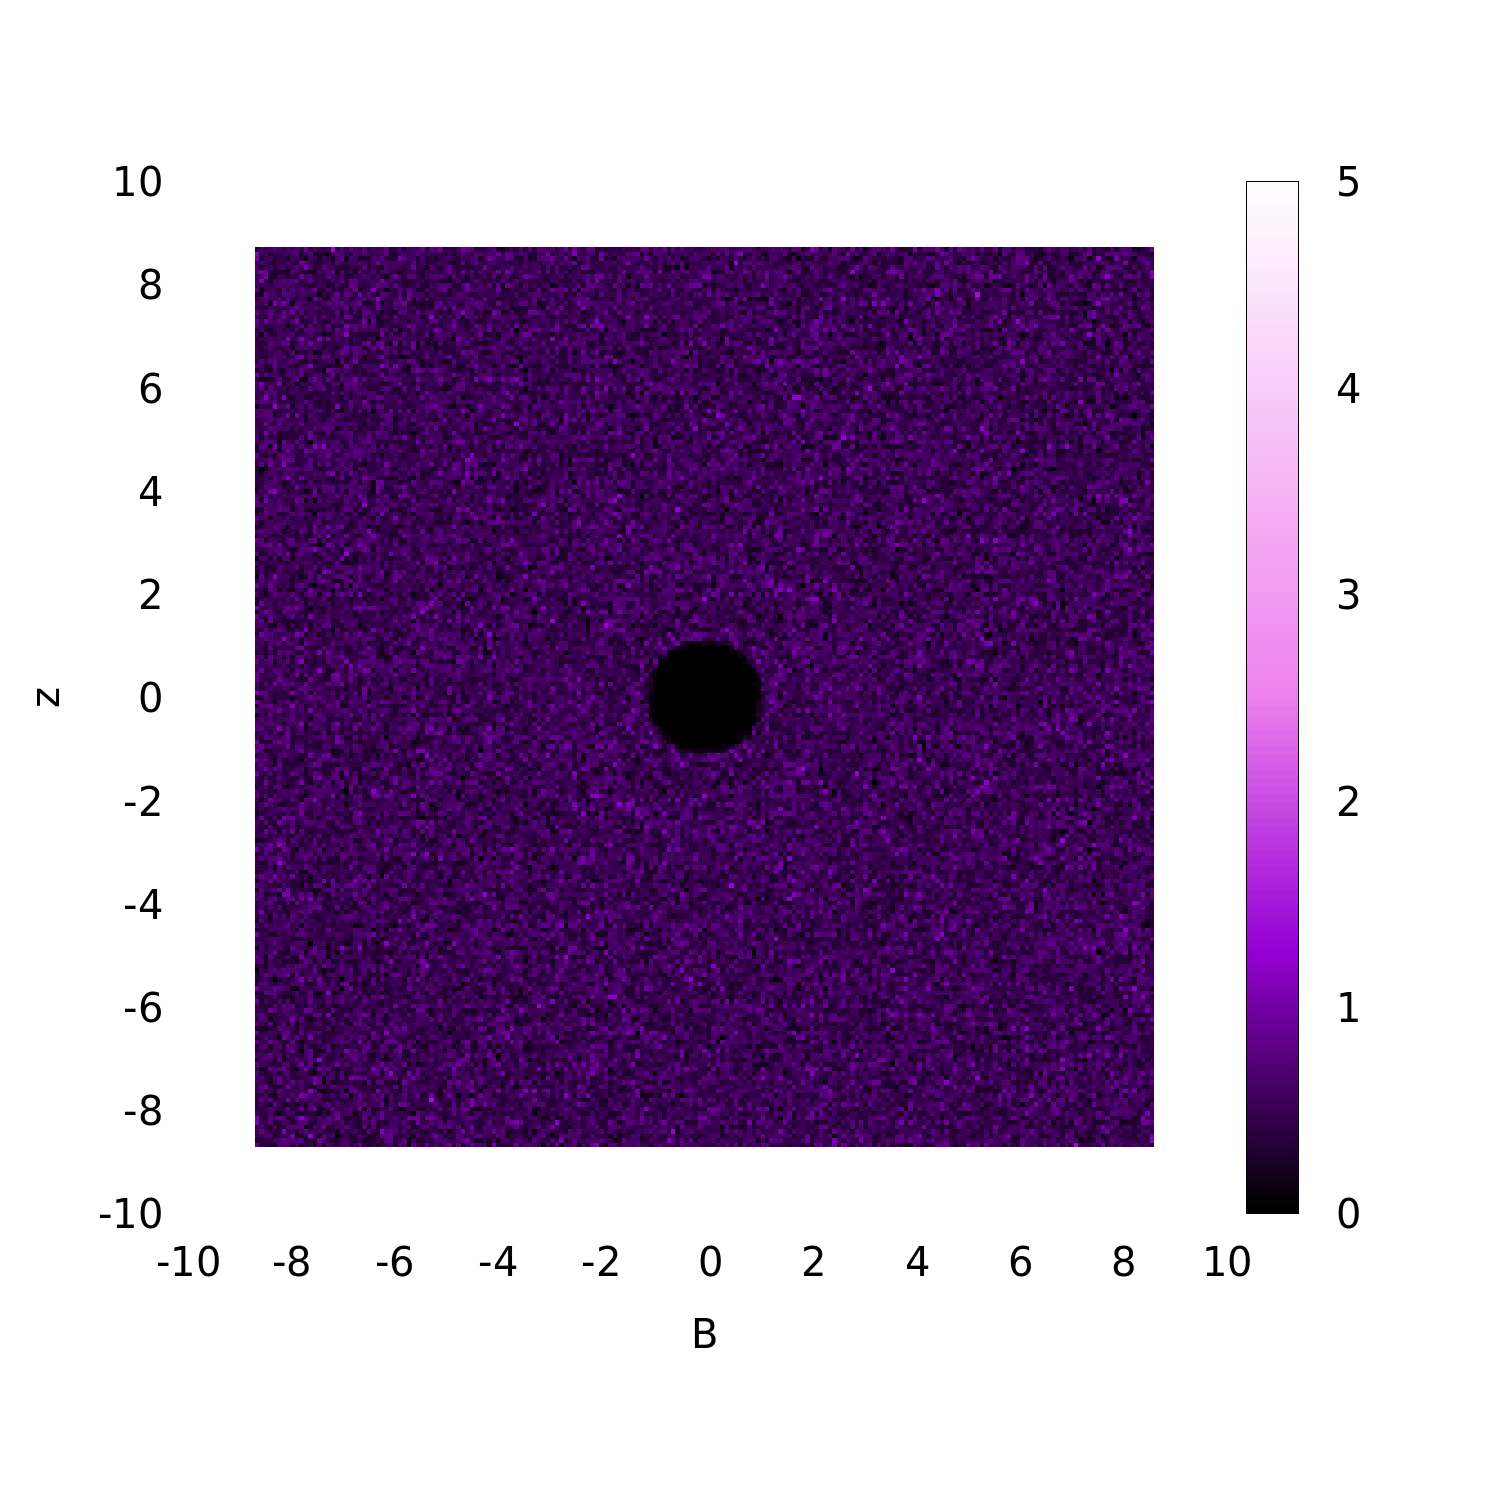
\includegraphics[width=0.5\columnwidth]{gyz_noB.png}
    \caption{Pair distribution function of HSCs without a magnetic field on the yz-plane at $\phi=0.50$.}\label{fig:gyz_noB}
\end{figure}
%\newpage


\section{Study of hematite-silica particle shape}
According to our computer simulations, the phase behavior under an external field is rather sensitive to particle shape, 
hence we carefully studied the shape of hematite-silica particles.
We obtained the 2D contours (as set of 2D points) of particles with aspect ratio $\rho_1 = 2.82$ and $\rho_2 = 3.69$ from 2D TEM images 
(see Figs. 1(a) and 1(b) in the manuscript). The coordinates of these points will be measured in pixels which have to be meant as 
arbitrary units.
Then, these contours were fitted by an ellipse ($\mathcal{F}_{e}$) and by the 2D curve which is obtained by projecting a spherocylinder 
onto a plane parallel to its symmetry axis ($\mathcal{F}_{s}$). Fits to $\mathcal{F}_{e}$ were performed by exploiting a recently 
developed and very efficient algorithm to find the roots of a quartic equation~\cite{DeMicheleACM}.
In the following, we will refer to latter curve also as 
``spherocylinder'' for the sake of simplicity.

If $\mathcal{C}$ is the set of 2D points which forms the contour of a particle, then we can define the distance $d$ between
$\mathcal{C}$ and $\mathcal{F}_\alpha$, with $\alpha\in\{e,s\}$, as follows:
\begin{equation}
  d \equiv \min_{\ontop{(x_c,y_c)}{(x_{fit}, y_{fit})}} \sqrt{{(x_c - x_{fit})}^2 + {(y_c - y_{fit})}^2}\label{eq:distdef}
\end{equation}
where $(x_c,y_c)\in \mathcal{C}$ and $(x_{fit},y_{fit})$ belongs either to $\mathcal{F}_e$ or $\mathcal{F}_s$.
Note that, if $d=0$ for a given particle, this means that this particle has a contour which is perfectly fitted
by the chosen shape (i.e.~either $\mathcal{F}_e$ or $\mathcal{F}_s$).

After having fitted all contours to both $\mathcal{F}_e$ and $\mathcal{F}_s$, we calculated according to 
Eq.~\ref{eq:distdef} the distances $d$, from which we built the histograms shown in Fig.~\ref{fig:Mean_dist}.
Since the particles are not symmetric with respect to their major axis, we obtained an estimate of $d$ from each of the two 
sides of each contours with respect of such axis (see Figs.~\ref{fig:Part_fit}(a) and~\ref{fig:Part_fit}(b)).
It can be seen that the more elongated particles ($\rho = 3.69$) are more ellipsoidal, being the average value of $d$ closer
to $0$ when particle contours are fitted by $\mathcal{F}_e$, than when they are fitted to $\mathcal{F}_s$ 
(see Fig.~\ref{fig:Mean_dist}(a)). On the contrary, the contours corresponding to particles with $\rho = 2.82$ exhibit 
an hybrid nature since their average distances to $\mathcal{F}_e$ and to $\mathcal{F}_s$ have comparable values
(see Fig.~\ref{fig:Mean_dist}(b)). 

%with a comparable mean distance distribution between the two fits.

\begin{figure}
    \centering
    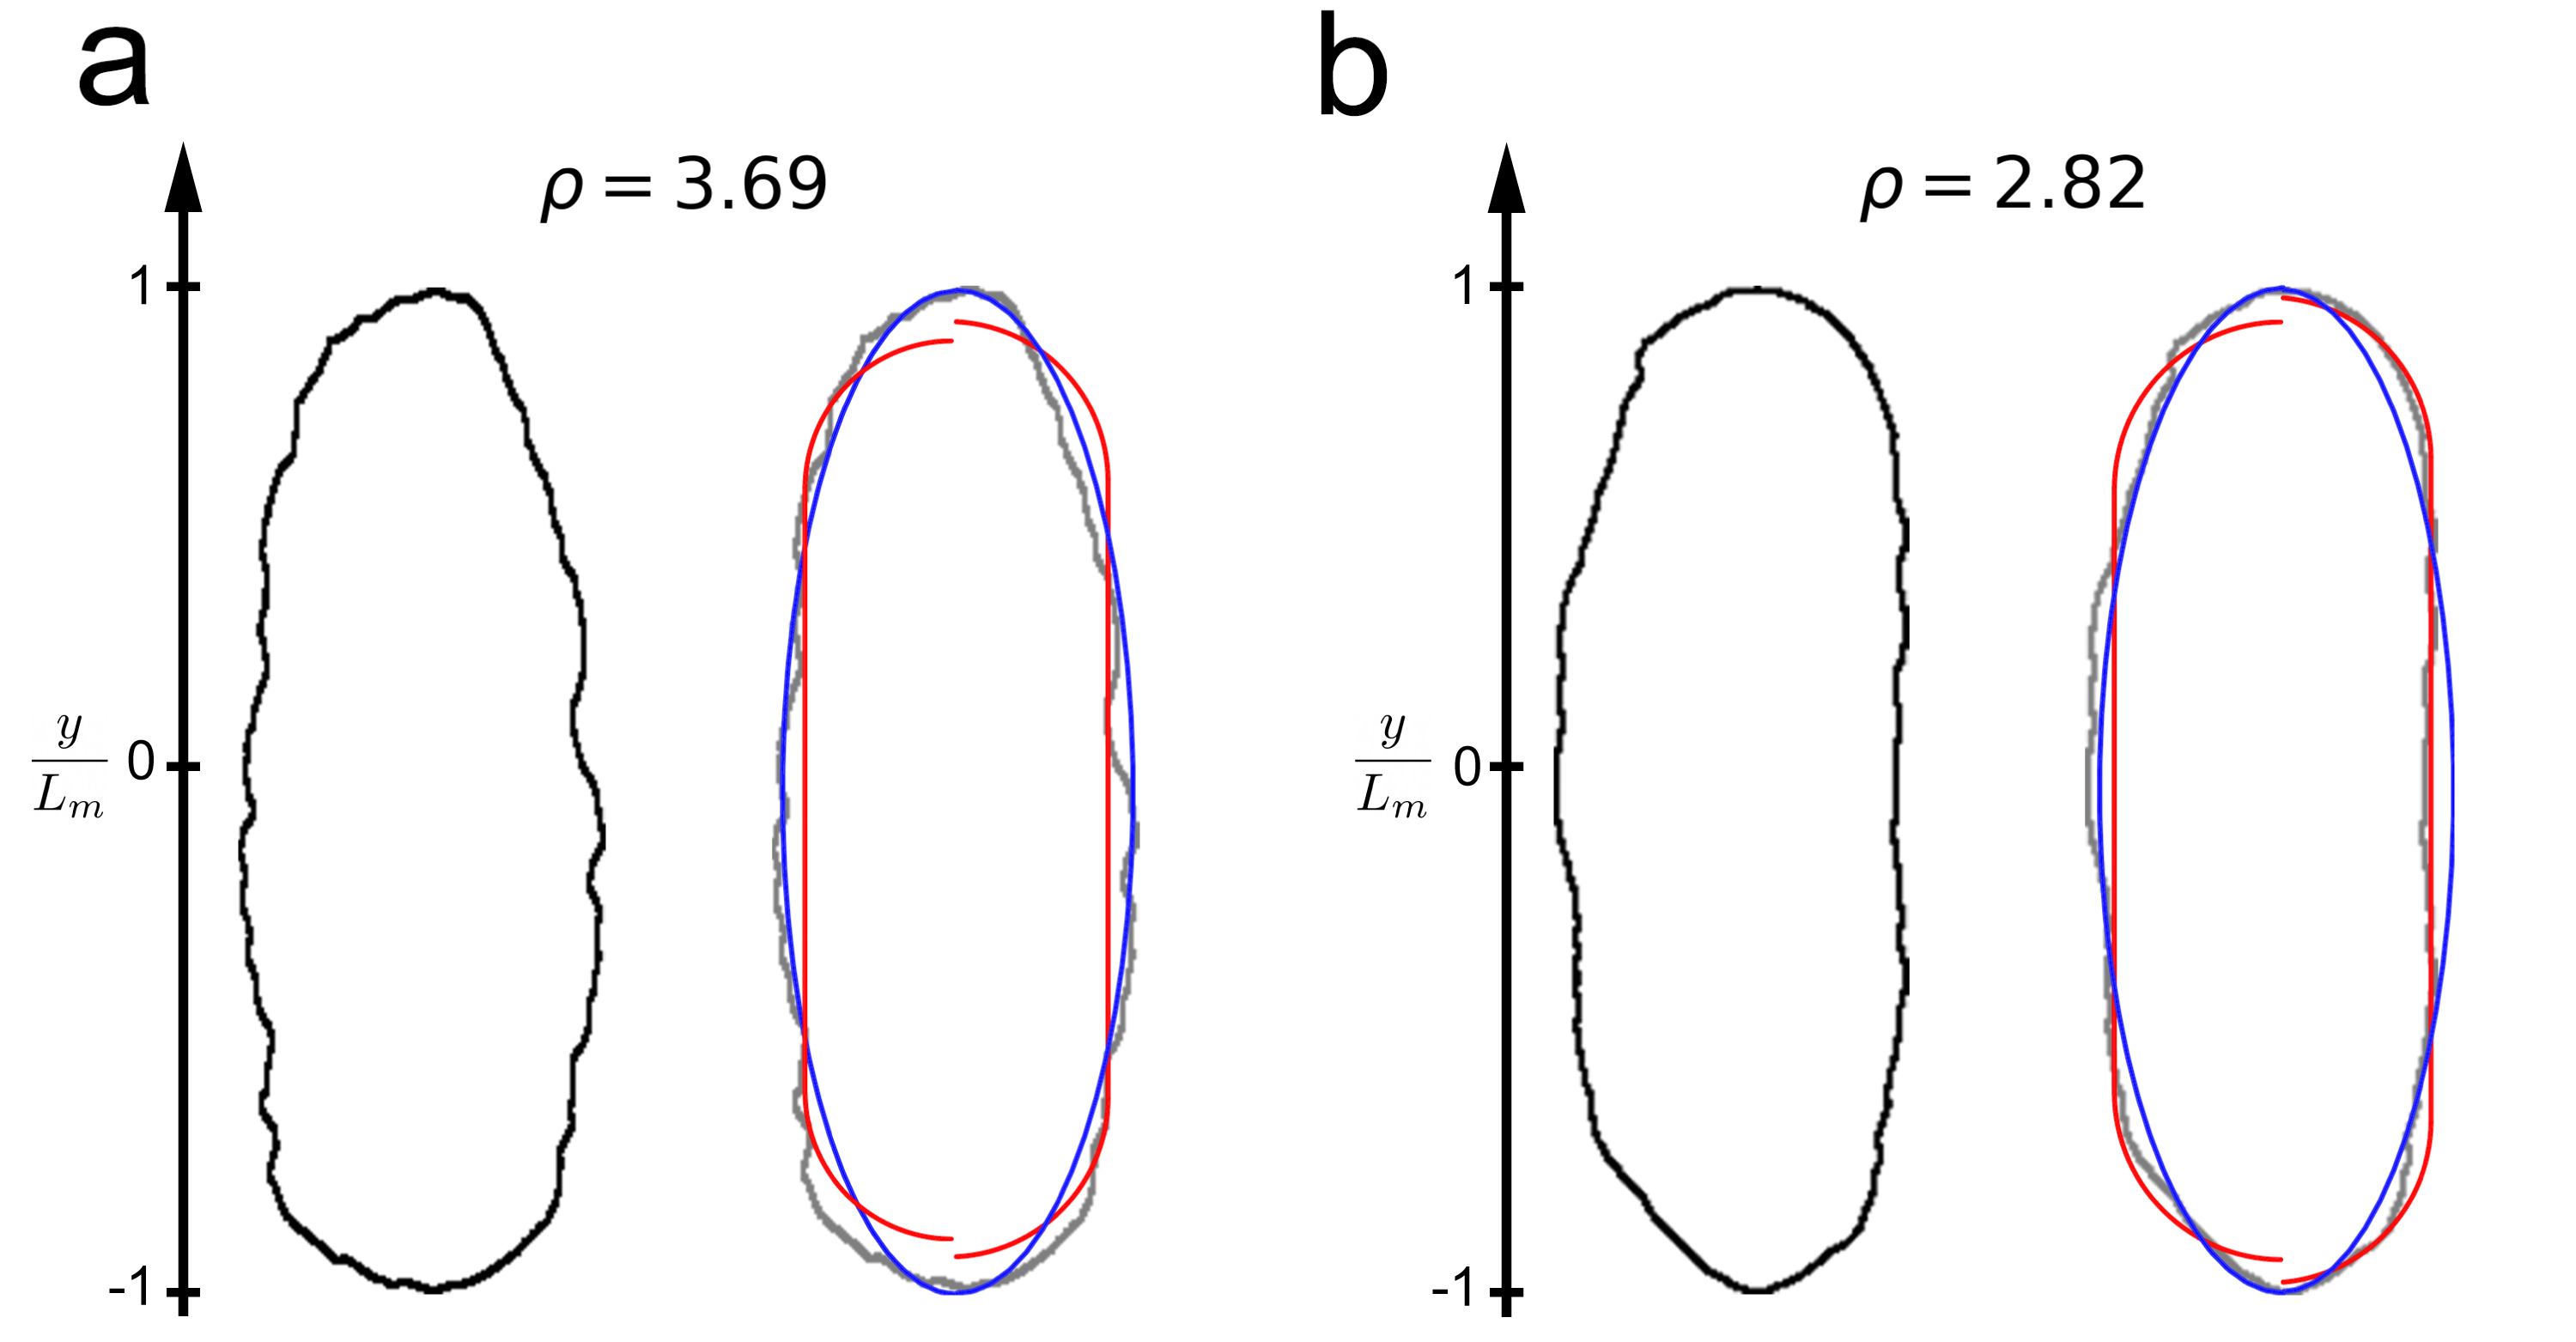
\includegraphics[width=0.95\columnwidth]{Part fit.png}
    \caption{Contours of particles with $\rho = 3.69$ (a) and $\rho = 2.82$ (b) has been fitted using an ellipse (in blue) and a 
    spherocylinder (in red).}\label{fig:Part_fit}
\end{figure}

\begin{figure}
    \centering
    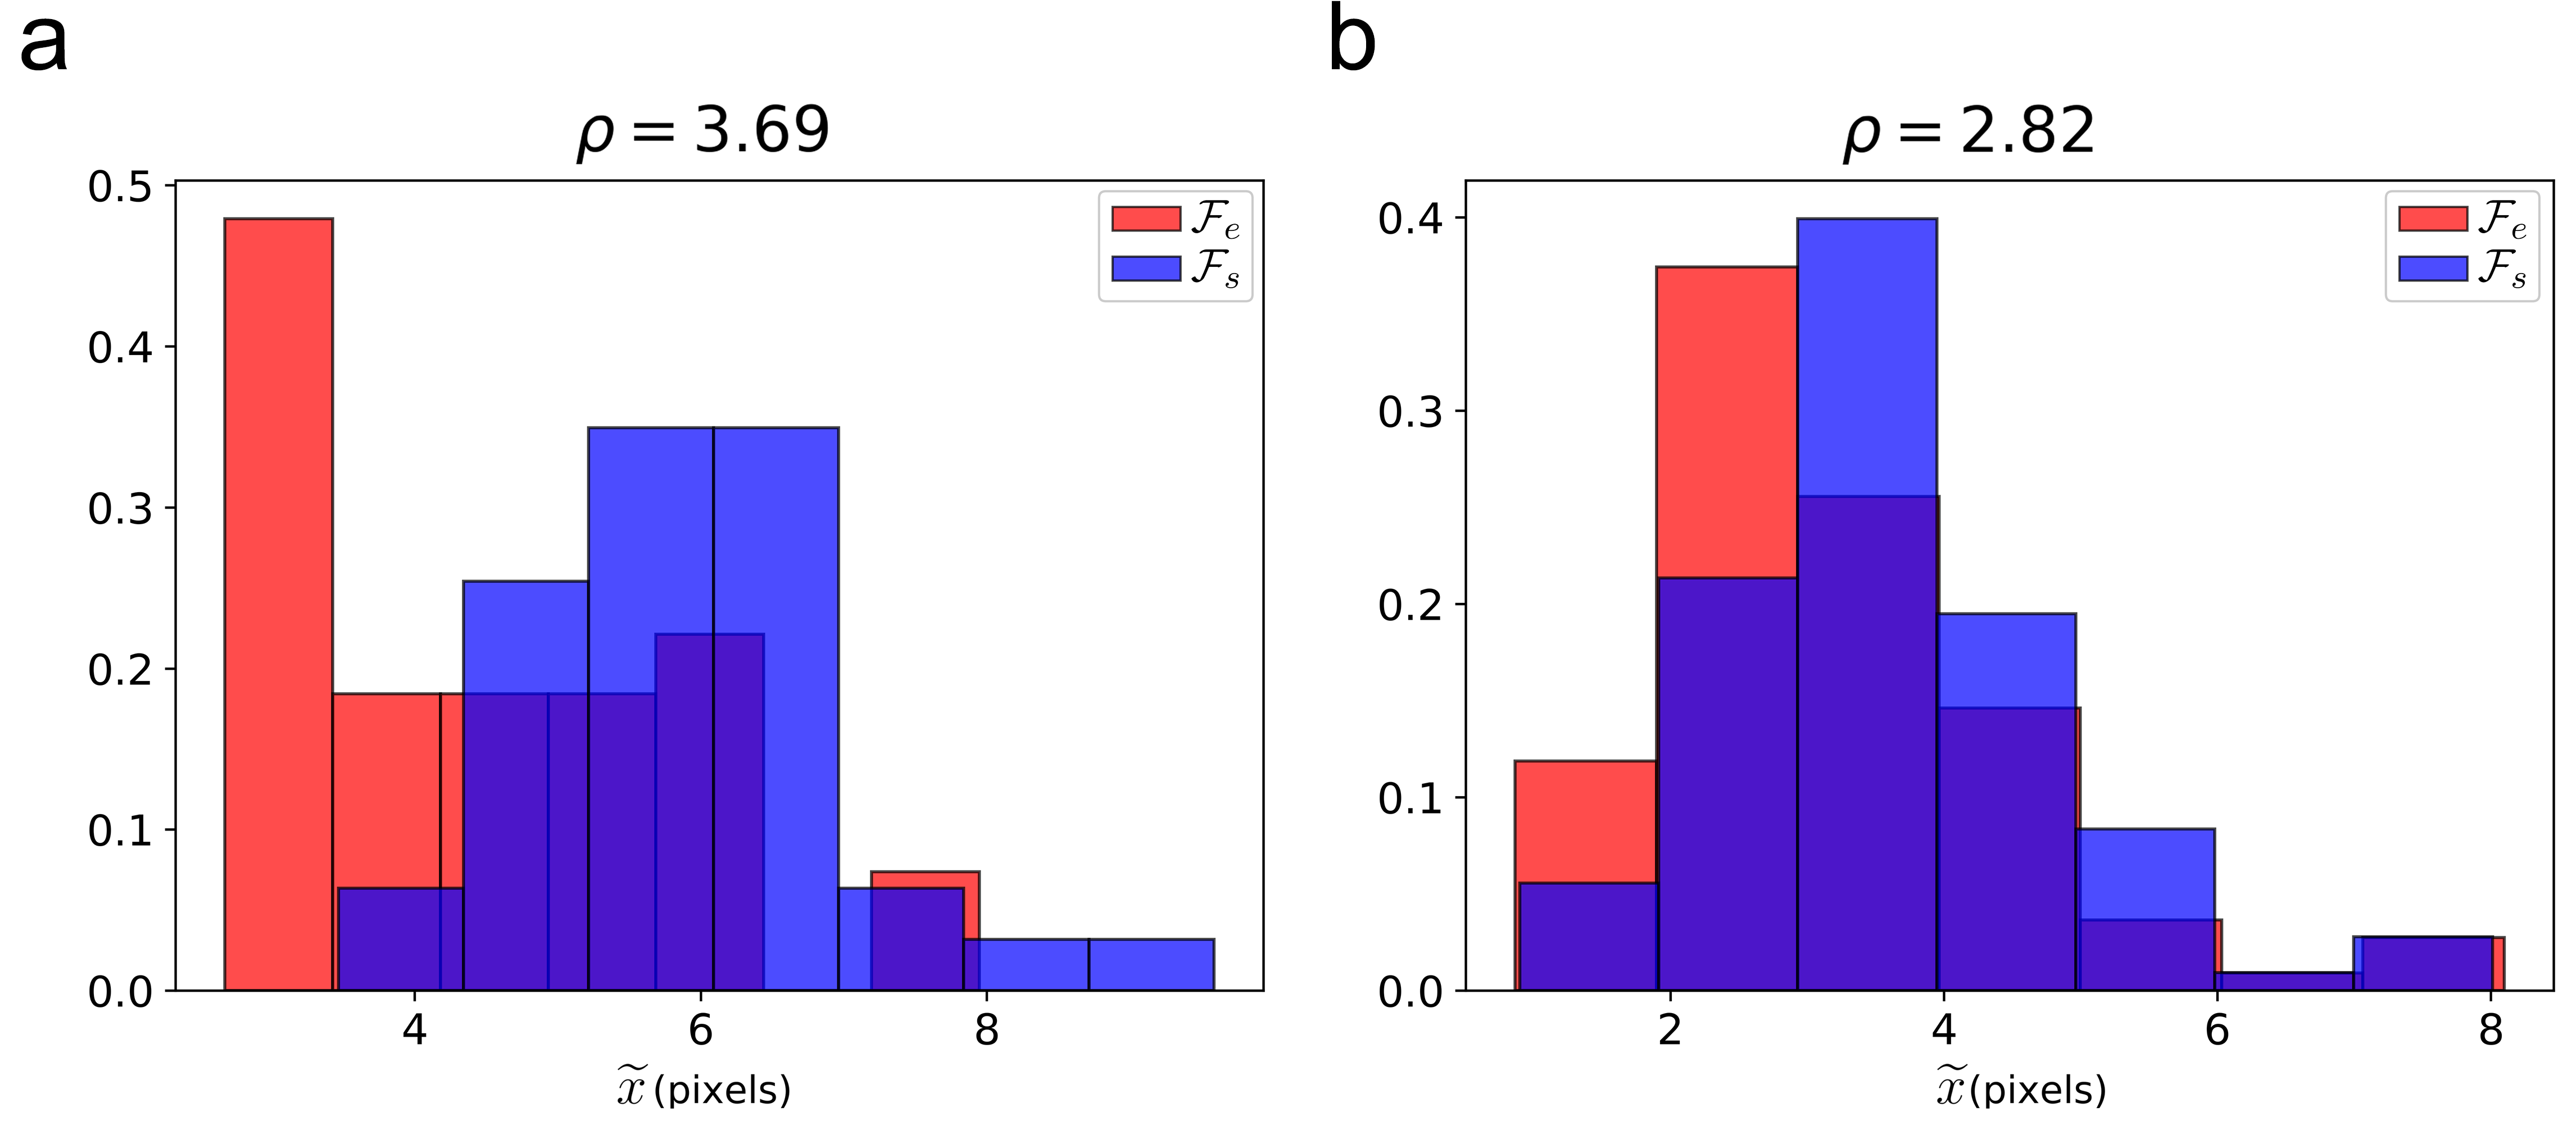
\includegraphics[width=0.95\columnwidth]{Mean_dist.png}
    \caption{Probability density of the distance $d$ for both fitting shapes $\mathcal{F}_e$ (ellipse) and $\mathcal{F}_s$ 
      (spherocylinder). (a) $\rho = 3.69$ and (b) $\rho = 2.82$.}\label{fig:Mean_dist}
\end{figure}

To further characterize the shape of particles, starting from the contours $\mathcal{C}$ of all particles, for both $\rho=3.69$
and $\rho=2.82$, we built the ``mean'' contour which is shown in Fig.~\ref{fig:Mean_bord}(a).
Then, we fitted these mean contours to $\mathcal{F}_s$ and $\mathcal{F}_e$ and we calculated for each point belonging to the 
contour the quantity:
\begin{equation}
  \widetilde{x}^2 = {(x_c - x_{fit})}^2 
\end{equation}
Figure~\ref{fig:Mean_bord}(b) shows $\widetilde{x}^2$ as a function of $y_c/L_m$ (normalized position), where $L_m$ is the 
length of the major axis of the mean contour.
% TODO: in Fig. S17 use a different name for the distance, show explicitly the reference system in Fig. S17 a 
% replace d^2 with \widetilde{x}^2 in Fig. S17

First note that values of $\widetilde{x}^2$ for the fits to $\mathcal{F}_e$ 
are on average much smaller than the ones for the fits to $\mathcal{F}_s$, 
thus suggesting that an ellipsoidal shape better reproduces the particle contours. Nevertheless, while for the fit of the 
mean contour to an ellipse ($\mathcal{F}_e$) $\widetilde{d}^2$ is on average larger for the less elongated particles ($\rho=2.82$) 
than for the more elongated ones (left panel of Fig.~\ref{fig:Mean_bord}(b)), 
the opposite behavior is observed for the fit of the mean contour to $\mathcal{F}_s$ (right panel of Fig.~\ref{fig:Mean_bord}(b)). 
Latter result highlights again the hybrid nature of particles with $\rho=2.82$ which, to some extent, are more spherocylinder-like 
than the ones with $\rho=3.69$.

\begin{figure}
    \centering
    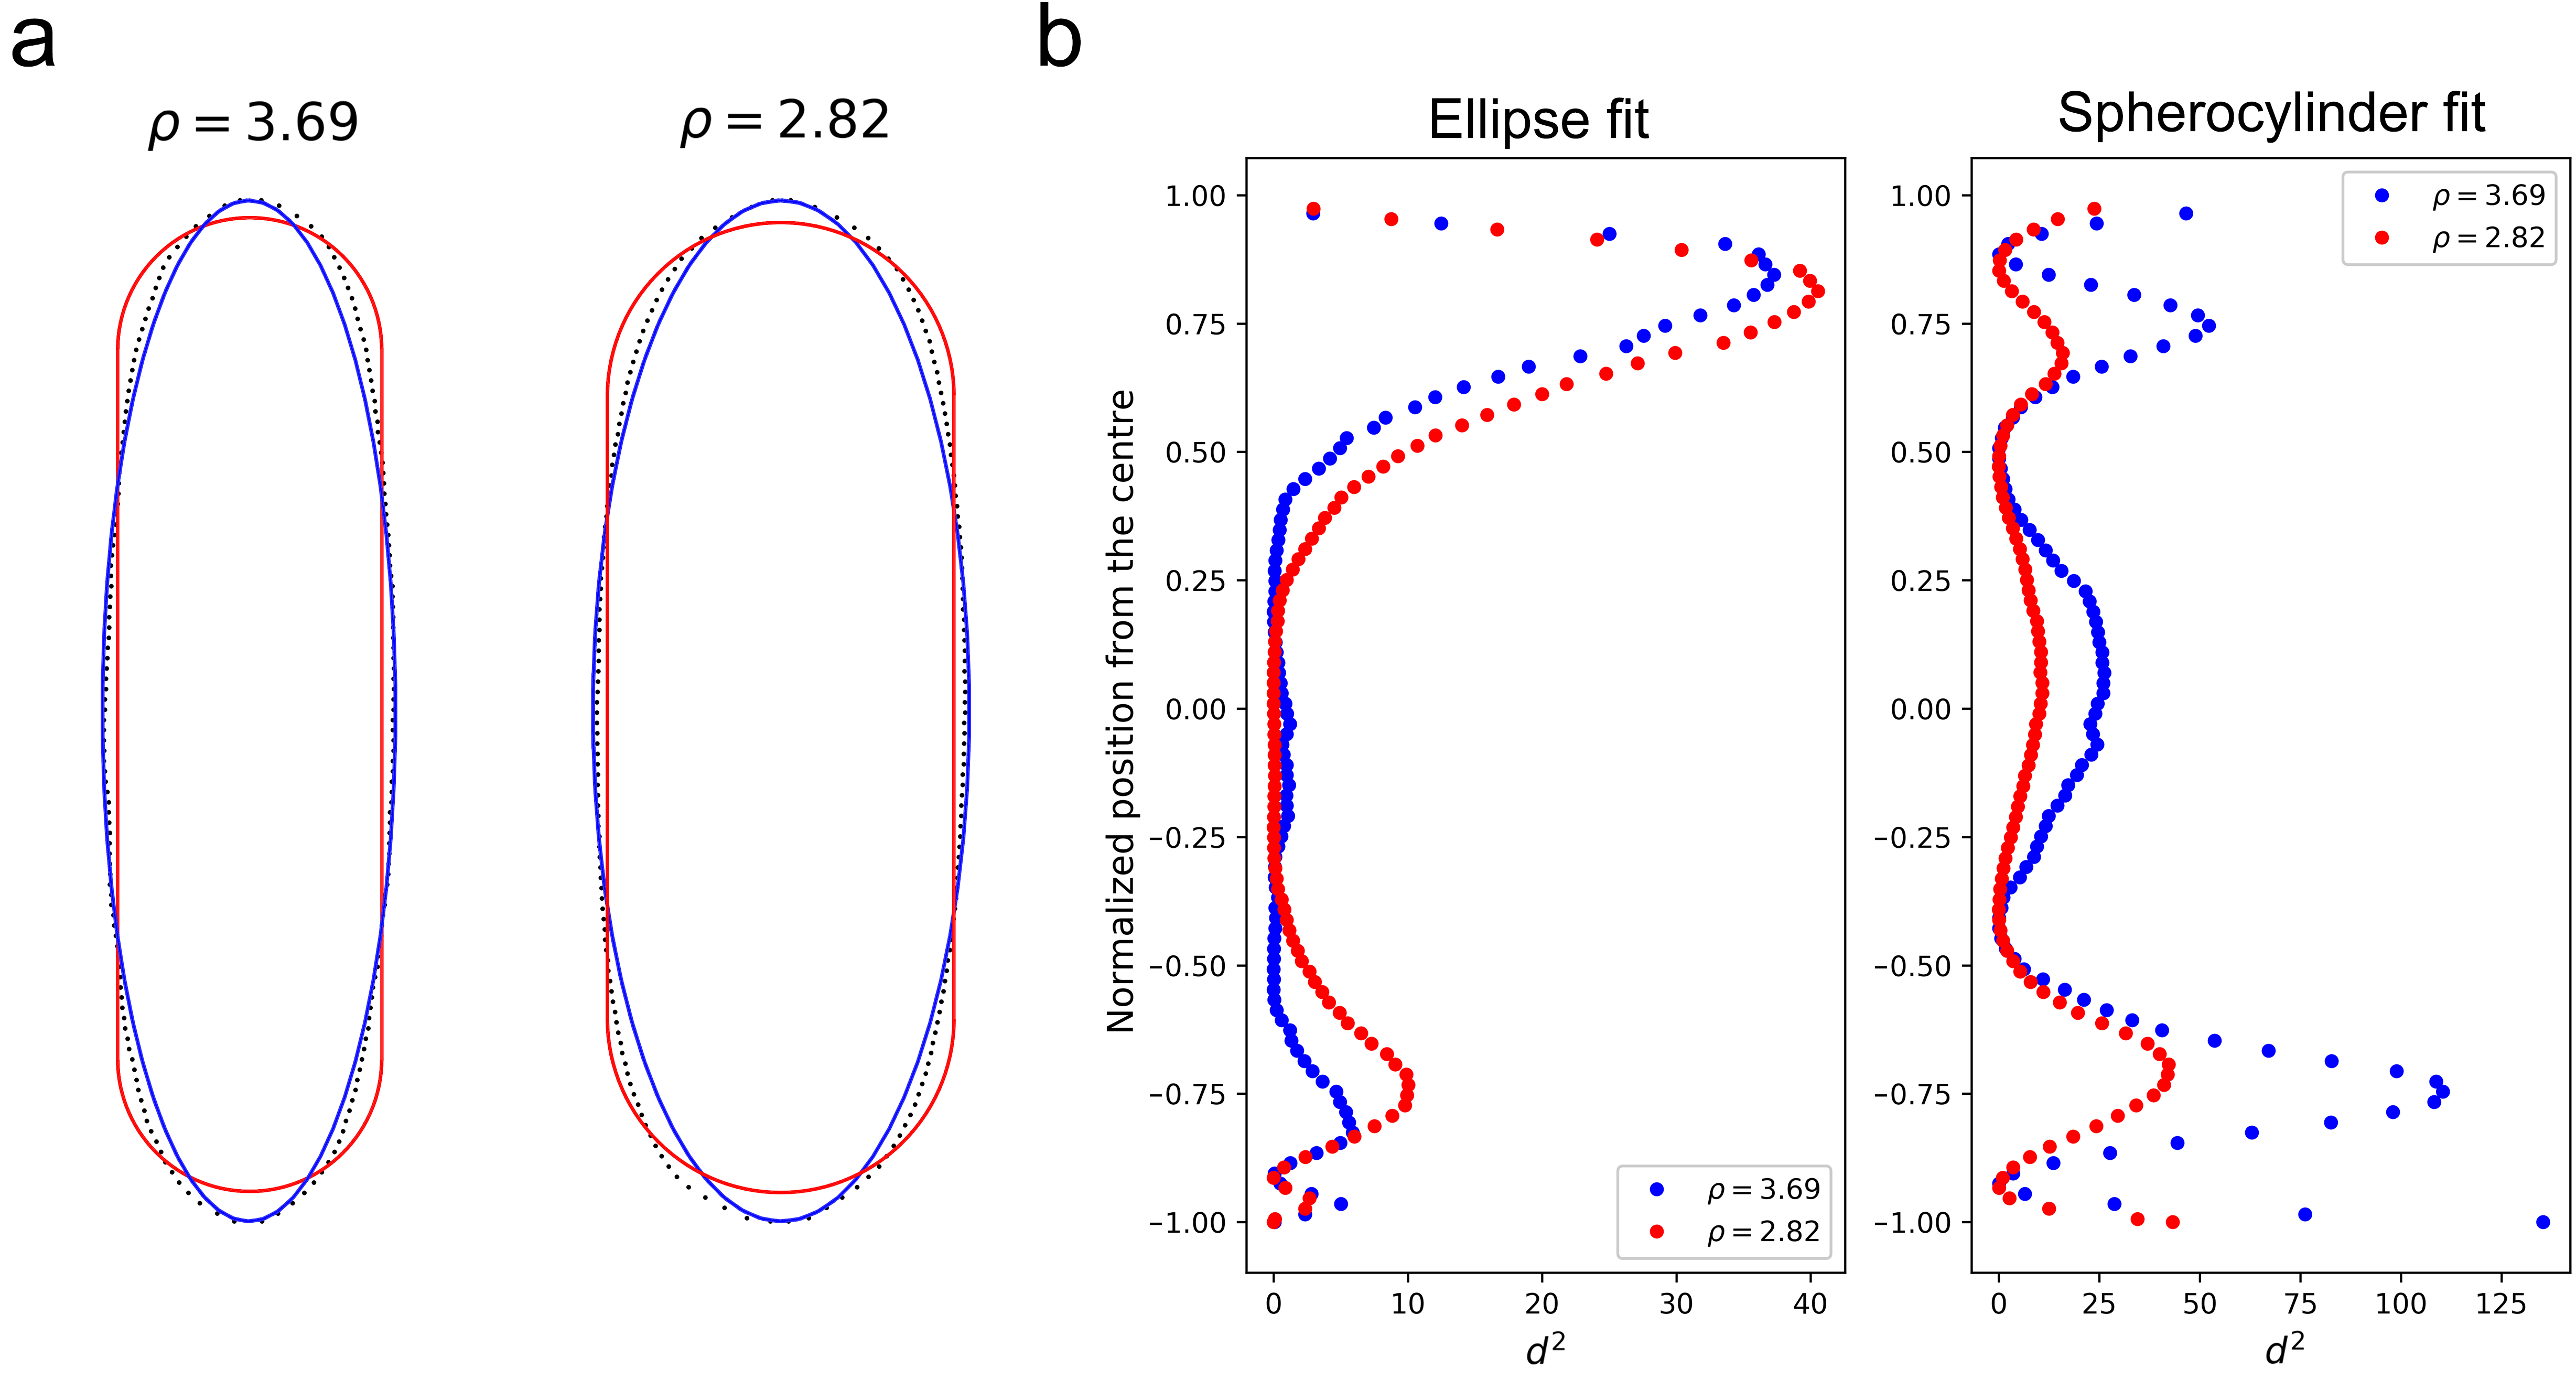
\includegraphics[width=0.7\columnwidth]{Mean_bord.png}
\caption{(a) Mean contour of the particles for both elongations (black dots) together with the fits to $\mathcal{F}_e$ and 
$\mathcal{F}_s$ (blue and red curve respectively). (b) $\widetilde{x}^2$ as a function of $y/L_m$.}\label{fig:Mean_bord}
\end{figure}

To better elucidate the hybrid nature of particles with $\rho=2.82$, in the following we will show that they
possess on average a more cylinder-like midsection than the ones with $\rho=3.69$. 
Hence, less elongated particles resemble more spherocylinders in their midsections, being them rather cylinder-like (i.e. ``flat'').

We performed a fit of the contours of each particle to a straight line parallel to their major axis of length $L$ (y-axis)
in the interval $[-l/2, l/2]$ (with $l < L$) and we calculated the average distance $d_f$ of
the particle's contour from the fitting line over such interval. 
We repeated latter procedure for several values of $l$ starting from $l=2/L$ up to a value $l_{max}$, such that
$d_f > 5$ (in units of pixels). $l_{max}$ quantifies the flatness of the midsection of the particles, in that 
the larger $l_{max}$ and the flatter can be considered the midsection of particles.

The result of this analysis can be found in Fig.~\ref{fig:maxlength_div}, where histograms of $l_{max}/L$ values are shown
for both elongations. Since the histogram is peaked around a larger value of $l_{max}/L$ for $\rho=2.82$, one can conclude
that less elongated particles have a larger cylinder-like (flat) midsection. 

\begin{figure}
    \centering
    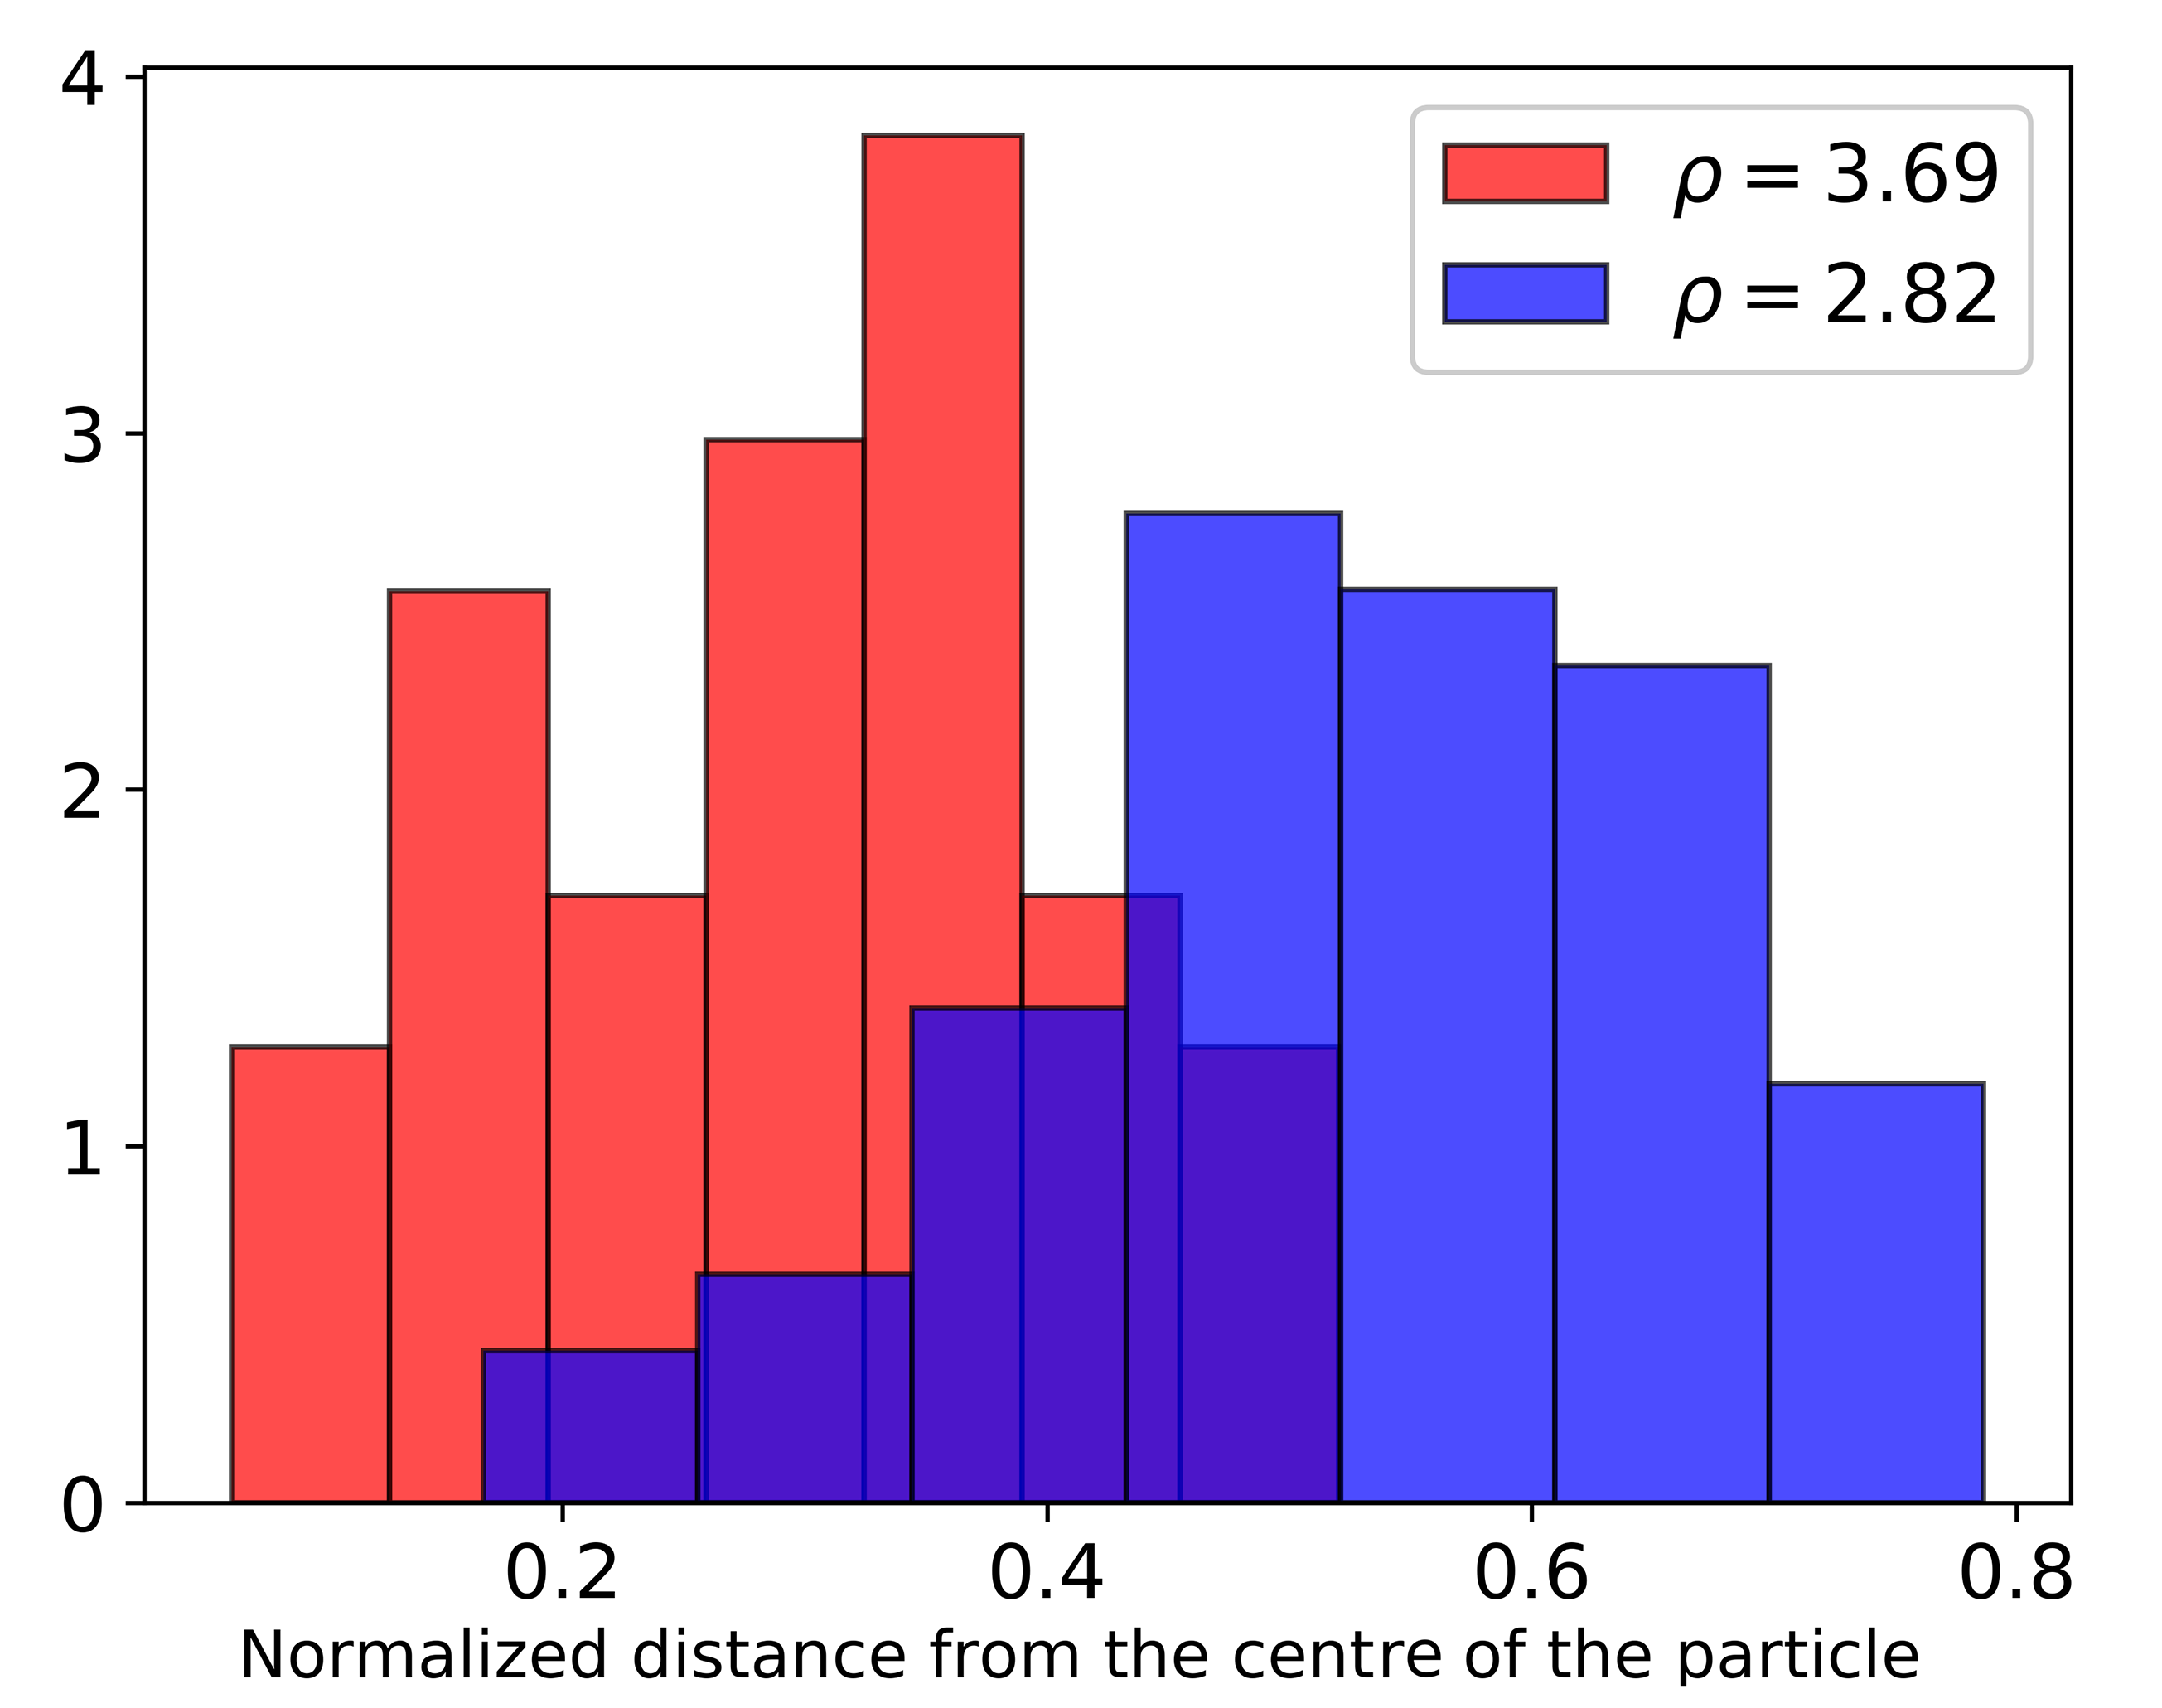
\includegraphics[width=0.5\columnwidth]{maxlength_div.png}
    \caption{Probability density for $l_{max}$ for both aspect ratios $\rho=3.69$ (red) and $\rho=2.82$ (blue).}\label{fig:maxlength_div}
\end{figure}

\bibliography{ref_dubble}


\end{document}
